\chapter{Introducción} \label{cap: introduccion}

Este capítulo se plantea como una introducción al presente proyecto y su campo de estudio: la fabricación aditiva (\acrshort{AM}). El capítulo se encuentra dividido en cuatro bloques fundamentales. El primer bloque está destinado a la definición de los procesos \acrshort{AM} comentando su origen y sus aplicaciones más innovadoras.

El segundo bloque corresponde al estado del arte y se encuentra dividido en tres secciones: la primera será la responsable de describir el flujo de trabajo general seguido por los procesos de fabricación aditiva más convencionales, la segunda sección introducirá los sistemas \acrshort{AM} robotizados presentando las tecnologías de mayor impacto y dando unas pinceladas sobre la labor de preparación de estaciones. Finalmente, la tercera sección se centrará de forma específica en los procesos \acrshort{NPAM}.

A partir de lo presentado en el estado del arte, el tercer bloque indicará las limitaciones encontradas en el estado del arte y servirá para definir la motivación del proyecto. Esta reflexión servirá para introducir el cuarto y último bloque dedicado a la presentación del marco de proyecto dentro del departamento de \hyperlink{https://fabricacion.industriales.upm.es/}{Ingeniería de Fabricación} de la ETSII-UPM.

\section{Fabricación aditiva}
La \acrfull{AM} es un conjunto de procesos de fabricación enfocados en la producción de componentes tridimensionales a partir de un diseño \acrshort{CAD} previo y la adición de capas de material sobre diferentes soportes. La fabricación aditiva supone un campo novedoso en el que se dispone de una mayor libertad de diseño. Es decir, no existen las limitaciones de otras de técnicas de fabricación que suelen emplear procesos de eliminación de material (conocidos en literatura como \acrfull{SM}).

Los procesos de fabricación sustractiva se caracterizan por crear un producto final retirando material del bloque. En ellos se busca obtener la pieza en el menor tiempo posible, con coste reducido, tolerancias dimensionales ajustadas y especificaciones de diseño fijadas de antemano. Durante mucho tiempo estos procesos han sido la piedra angular de la industria manufacturera, siendo la opción  preferida para procesos a gran escala. Sin embargo, la retirada de material trae problemas de cara al prototipado y al ensayo de ciertas geometrías. La posibilidad de ahorrar los costes asociados a este tipo de operaciones ha servido como puerta de entrada de la \acrshort{AM} a sectores de mayor escala.

\begin{figure}[h!]
    \centering
    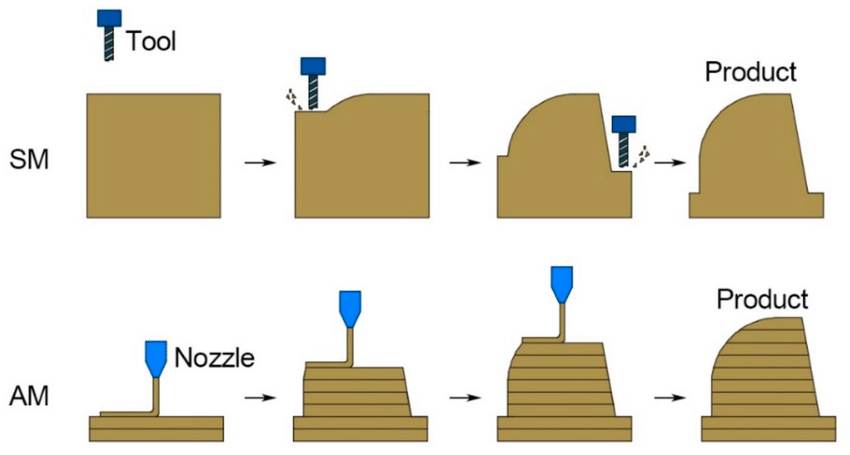
\includegraphics[scale=0.25]{figuras/sm_vs_am.png}
    \caption{Fabricación aditiva frente a sustractiva \cite{Tao2021}}
    \label{fig:aditiva_vs_sustractiva}
\end{figure}

Las técnicas de \acrshort{AM}, son idóneas para el desarrollo de piezas más personalizadas, la optimización de material, la reducción de residuos o la construcción de diseños de alta precisión y con geometrías complejas \cite{Li_2020} \cite{Rashid_2024}\cite{Loyda_2023}. No obstante, estos procesos son más lentos al requerir de métodos posteriores de limpieza, curado y acabado \cite{AMvsSM_Dasult}. En la figura \ref{fig:aditiva_vs_sustractiva} se muestra esquemáticamente el enfoque que aborda cada método de fabricación para una misma geometría. 

\subsection{Historia de la fabricación aditiva}
Los primeros registros de técnicas de fabricación aditiva son gracias al japonés Hideo Kodama, del Instituto Municipal de Investigación Industrial de Nagoya. En su trabajo publicado en 1981 \cite{Kodama1981}, Kodama habla de sus experimentos realizados con una resina fotosensible. Dicha resina se solidificaba en regiones concretas de un \textit{plotter} XY con ayuda de una matriz de haces de luz ultravioleta. Kodama pudo describir esta nueva tecnología con hasta tres métodos diferentes, los cuales se muestran la Figura \ref{fig:metodos_Kodama1981}. En dicho trabajo ya se comenzaron a mencionar términos que hoy en día ya son comunes en el mundo de la fabricación aditiva como pueden ser: \textit{altura de capa}, \textit{geometría de soporte} o \textit{viscosidad de resina}. 

\begin{figure}[h!]
    \centering
    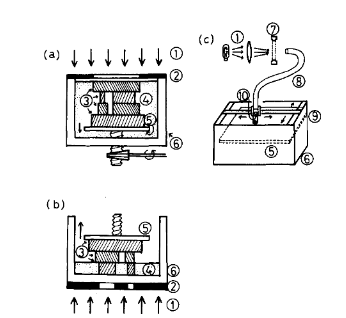
\includegraphics[scale=0.5]{figuras/metodos_Kodama1981.png}
    \caption{Métodos descritos por Kodama \cite{Kodama1981}.}
    \label{fig:metodos_Kodama1981}
\end{figure}

Poco tiempo después -en 1984- el norteamericano Charles Hull desarrollaría la técnica de \acrfull{SLA}. La \acrlong{SLA} utilizaba polímeros sensibles a la luz que se depositaban por capas sobre una cama móvil. Los primeros trabajos de Hull se trataban de versiones miniaturizadas de objetos diseñados con \acrshort{CAD}. Dichos diseños podían fabricarse rápidamente y se utilizaban en labores de prototipado. El éxito fue tan grande que dio origen a su propia familia de procesos \acrshort{AM} (los \acrshort{VPP}) y además permitió a Hull fundar la primera compañía de fabricación aditiva de la historia: 3DSystems \cite{web_3DSystems}. En la figura \ref{fig:patente_sla} se muestra el primer modelo de estereolitografía. \label{sec:esterilitografia}

\begin{figure}[h!]
    \centering
    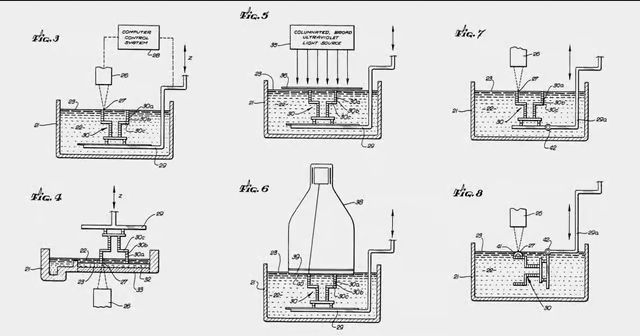
\includegraphics[scale=0.30]{figuras/patente_sla.png}
    \caption{Primer modelo de \acrshort{SLA} patentado \cite{Hull1984}.}
    \label{fig:patente_sla}
\end{figure}

El proceso de fabricación aditiva más conocido es el de \acrfull{MEX}, cuyo primer desarrollo corrió a cargo del ingeniero Scott Scrump en 1989 \cite{Scrump1989}. En el año 2005, las patentes de Scrump (Figura \ref{fig:patente_scrump}) fueron liberadas y el desarrollo de nuevas máquinas \acrshort{AM} tuvo un auge nunca antes visto gracias a la proliferación de movimientos basados en el código abierto como RedRap (Figura \ref{fig:maquina_redrap1}) \cite{web_RedRap}. Iniciativas de este tipo han permitido que la fabricación aditiva haya podido llegar a multitud de empresas y hogares, favoreciendo la inversión y la aparición de nuevas tecnologías derivadas.

\begin{figure}[h!]
    \centering
    \begin{subfigure}[h]{0.45\linewidth} 
        \centering
        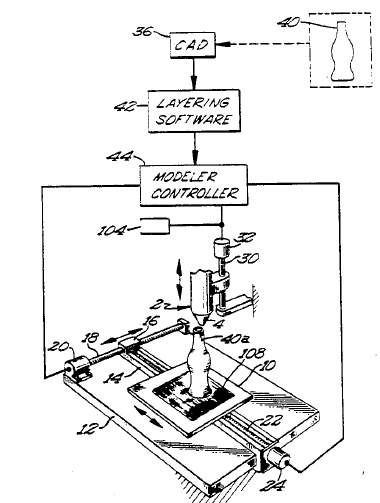
\includegraphics[scale=0.38]{figuras/patente_scrump.png}
        \caption{Sistema \acrshort{MEX} \cite{Scrump1989}.}
        \label{fig:patente_scrump}
    \end{subfigure}
    \begin{subfigure}[h]{0.45\linewidth} 
        \centering
        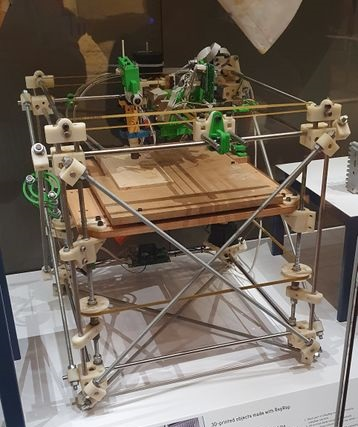
\includegraphics[scale=0.3]{figuras/maquina_redrap1.jpg}
        \caption{Primera máquina RedRap \cite{web_RedRap}.}
        \label{fig:maquina_redrap1}
    \end{subfigure}
    \caption{Comienzos de la \acrshort{MEX}}
    \label{fig:FDM_y_redrap}
\end{figure}

\subsection{Aplicaciones de la fabricación aditiva}
En los últimos años la \acrshort{AM} ha permitido el desarrollo de piezas altemente personalizadas con una variedad de materiales como madera, aleaciones metálicas, cerámicas o polímeros de diferentes propiedades. Esto es, se ha pasado de ser un campo centrado fundamentalmente en el prototipado de piezas, al diseño de elementos complejos de gran precisión y adaptabilidad. Algunos ejemplos de los sectores de aplicación más representativos son:

\begin{itemize}
    \item \textbf{Transporte aeroespacial}\\
    La AM es especialmente útil en aplicaciones que suponen un compromiso entre el volumen de producción y las exigencias técnicas. En este caso, los materiales más empleados son diferentes aleaciones metálicas. Estas aleaciones se utilizan para soportar las condiciones de críticas de presión y temperatura de ciertos componentes como motores a reacción o fuselaje de aviones \cite{BlakeyMiner2021}. En la figura \ref{fig:am_aplicaciones_aerol} se observa un prototipo a escala de un motor a reacción realizado mediante estas técnicas.
    
    \item \textbf{Automoción}\\
    La industria del automóvil sigue una línea similar a la aeroespacial. En este caso, las aplicaciones más notables se encuentran focalizadas en la optimización de material. Con ayuda de estos sistemas, se obtiene un prototipo impreso y, si los ensayos son exitosos, existe la posibilidad de disponer el modelo final en una matriz de impresión \cite{Zhao_2023}. La figura \ref{fig:am_aplicaciones_automovil} ilustra un ejemplo, a la izquierda se presenta el diseño original y la derecha el resultante de la optimización topológica, ambos hechos con \acrshort{AM}.
    
    \begin{figure}[h!]
        \centering
        \begin{subfigure}[h]{0.45\linewidth} 
            \centering
            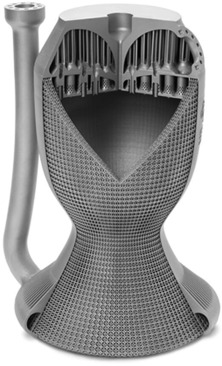
\includegraphics[scale=0.4]{figuras/am_aplicaciones_aero.jpg}
            \caption{Prototipo de motor a reacción \cite{BlakeyMiner2021}}
            \label{fig:am_aplicaciones_aerol}
        \end{subfigure}
        \begin{subfigure}[h]{0.4\linewidth} 
            \centering
            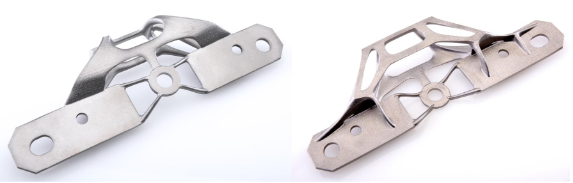
\includegraphics[scale=0.45]{figuras/am_aplicaciones_automovil.png}
            \caption{Bastidor hecho con \acrshort{AM} \cite{Zhao_2023}.}
            \label{fig:am_aplicaciones_automovil}
        \end{subfigure}
        \caption{Sector aeroespacial y automovilístico}
        \label{fig:FDM_y_redrap}
    \end{figure}

    \item \textbf{Sistemas electrónicos}\\
    Una de las ventajas más destacadas de la fabricación aditiva en el ámbito de los componentes electrónicos es su capacidad para delinear con precisión las diferentes regiones portadoras de electrones en componentes activos como diodos, transistores, amplificadores operacionales, y transistores bipolares de puerta aislada (IGBT) entre otros \cite{Bellacicca2018}\cite{Zhang2015}. Esta precisión a escala de micras es fundamental para garantizar el rendimiento óptimo de los dispositivos electrónicos, ya que permite un control más preciso del flujo de corriente eléctrica y facilita la integración de componentes en sistemas más complejos.
    
    Gracias a esta ventaja, la fabricación aditiva ha resultado de gran importancia para el descenso de los costes de la electrónica industrial y de consumo. La figura \ref{fig:am_aplicaciones_electronica} muestra un sensor luminoso con un amplificador operacional fabricado mediante esta técnica.

    \item \textbf{Diseño de materiales}\\
    La investigación en nuevos materiales va dirigida en los últimos años hacia métodos de fabricación que incluyan aleaciones con composición variable según el gradiente de tensiones. Los resultados más notables se han alcanzado con aleaciones que disponen de Ni y  Ti como principales constituyentes \cite{Li2019}. Otro campo interesante es la conocida como \textit{impresión 4D} \cite{Mahmood2023}, esto es, la impresión 3D de materiales cuyas propiedades cambian ante estímulos térmicos, eléctricos o luminosos. La figura \ref{fig:am_aplicaciones_materiales} muestra el cambio de forma de varios componentes hechos con AM ante elevadas temperaturas.

    \begin{figure}[h!]
        \centering
        \begin{subfigure}[h]{0.45\linewidth} 
            \centering
            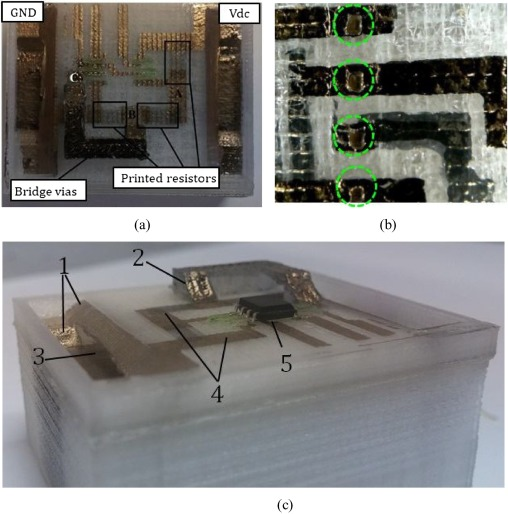
\includegraphics[scale=0.3]{figuras/am_aplicaciones_electronica.jpg}
            \caption{Sensor luminoso impreso en 3D \cite{Bellacicca2018}.}
            \label{fig:am_aplicaciones_electronica}
        \end{subfigure}
        \begin{subfigure}[h]{0.45\linewidth} 
            \centering
            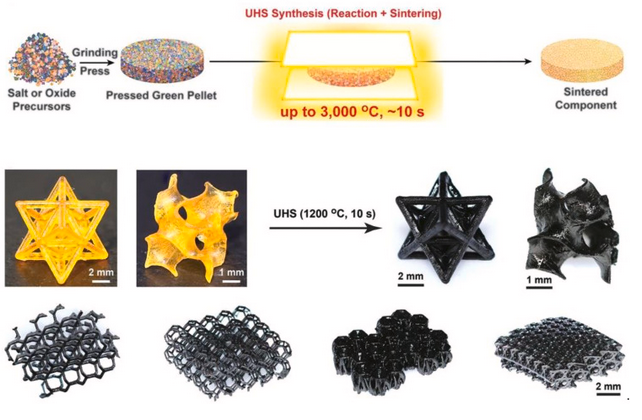
\includegraphics[scale=0.25]{figuras/am_aplicaciones_materiales.png}
            \caption{Demostración de composite hecho con impresión 4D \cite{Mahmood2023}.}
            \label{fig:am_aplicaciones_materiales}
        \end{subfigure}
        \caption{Fabricación electrónica y nuevos materiales}
        \label{fig:FDM_y_redrap}
    \end{figure}
    
    \item \textbf{Sector médico}\\
    La fabricación aditiva está ganado un rol de especial importancia en las especialidades médico-quirúrgicas. Algunas de las especialidades más demandadas son neurocirugía \cite{Guarino2021}, cirugía oral y maxilofacial \cite{Zoabi2022} o cirugía cardiaca \cite{Vukicevic2017}. Como norma general, los materiales más utilizados en estas aplicaciones son polímeros como \acrshort{ABS} y \acrshort{PLA} o resinas mezcladas con polvos cerámicos \cite{Kumar2021}. Cualquier aplicación de la \acrshort{AM} en este campo debe tener en cuenta siempre un condicionante: la no interferencia con pruebas diagnósticas en las que se irradie algún tipo de energía como pueden ser rayos X o imágenes de resonancia magnética. 
    
    La figura \ref{fig:am_aplicaciones_medico} muestra una reconstrucción de mandíbula hecha con un proceso \acrshort{AM}. Se ha empleado una imagen diagnóstica para elaborar una fédula personalizada para un caso clínico con el mentón completamente fracturado. A través de distintas iteraciones se pudo desarrollar un implante que resultase cómodo para el paciente y redujese el tiempo de operación.

    \begin{figure}[h!]
        \centering
        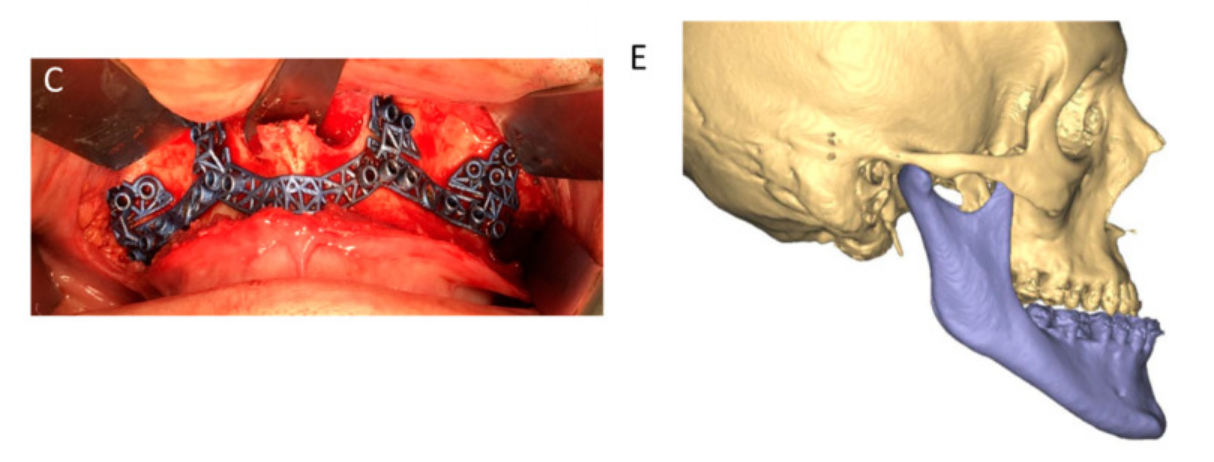
\includegraphics[scale=0.25]{figuras/am_aplicaciones_medico.png}
        \caption{Fédula mentoniana para reconstrucción de mandíbula \cite{Zoabi2022}.}
        \label{fig:am_aplicaciones_medico}
    \end{figure}
\end{itemize}

\section{Estado del arte}
Esta sección sirve para establecer un resumen de los últimos avances realizados en el campo de la fabricación aditiva robotizada, haciendo un especial hincapié en los modelos de geometrías no planares. Para ofrecer una perspectiva sencilla de comprender y centrar el enfoque en el desarrollo de una arquitectura de estación de este tipo, se establecen tres puntos principales.

El primer punto describirá el funcionamiento básico de un sistema de fabricación aditiva y describirá el flujo de trabajo que acompaña a este tipo de procesos. El segundo introducirá al lector en las tecnologías \acrshort{AM} robotizables mencionando aquellas con más facilidad para integrar este tipo de equipos, indicando las operaciones de mayor importancia y presentando algunas de las arquitecturas informáticas de estación robotizadas que han servido de referencia para este trabajo. El tercer y último punto se enfocará en la presentación de las tecnologías \acrshort{NPAM}. En él se comentarán sus principales ventajas y limitaciones, así como también pueden verse favorecidas por la integración de equipos robóticos en su flujo de trabajo.

\subsection{Fabricación aditiva convencional}
\subsubsection*{Funcionamiento básico}
\hypertarget{Funcionamiento básico}{}
\bookmark[level=subsubsection,dest=Funcionamiento básico]{Funcionamiento básico}

Como se ha indicado en líneas anteriores, la fabricación aditiva convencional utiliza un extrusor de material que termina depositándose sobre una cama plana.  El extrusor puede desplazarse en las configuraciones cinemáticas del espacio cartesiano (ejes XYZ) mientras la cama de impresión\footnote{Superficie sobre la que se va depositando el material} permanece quieta, o puede combinar su movimiento con el de un soporte móvil.

En las tecnologías \acrshort{MEX} convencionales, el material se encuentra inicialmente en forma de filamento flexible y para depositarse sobre la cama de impresión debe estar en un estado viscoso y fácilmente maleable. El mecanismo que aporta el calor y la presión necesarios para que tome esa consistencia es el extrusor. El extrusor se encuentra conectado a una pequeña unidad de cómputo que posee capacidad para determinar parámetros como: posición del extrusor, temperatura del material y velocidad de deposición del filamento.

Comúnmente se considera a las impresoras 3D comerciales como los ejemplos típicos de las tecnologías \acrshort{AM} tradicionales. El auge de este tipo de equipos ha permitido que cada fabricante desarrolle su propia variante de la estrategia propuesta. En la figura \ref{fig:impresora3d_1} se observa una estación de impresión 3D comercial, en la que el fabricante ha optado por un extrusor móvil en la dirección vertical y una horizontal, con una cama con movilidad en la dirección horizontal restante. La figura \ref{fig:impresora3d_2} muestra otra estación comercial, en este caso la cama permanece inmóvil y el extrusor es el único elemento móvil.

\begin{figure}[h!]
     \begin{subfigure}[h]{0.45\linewidth} 
        \centering
        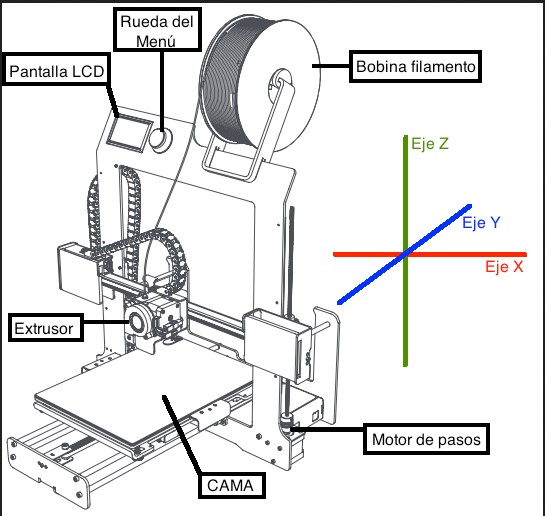
\includegraphics[scale=0.4]{figuras/impresora3d_1.jpg}
        \caption{Impresora 3D con extrusor y cama móvil \cite{GobCanarias}.}
        \label{fig:impresora3d_1}
    \end{subfigure}
    \begin{subfigure}[h]{0.45\linewidth} 
        \centering
        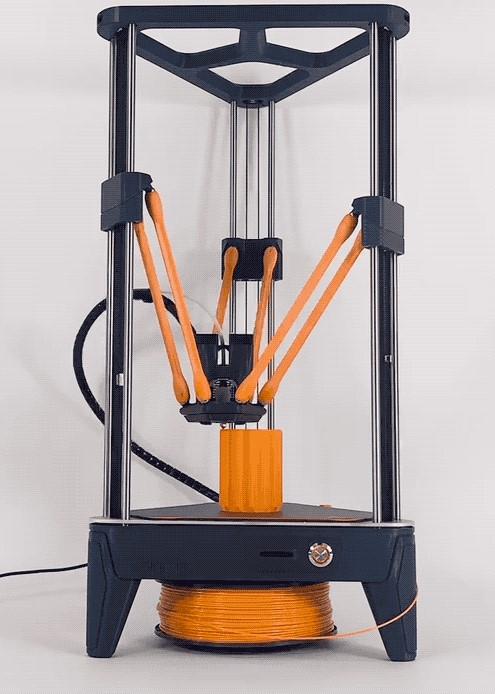
\includegraphics[scale=0.3]{figuras/impresora3d_2.jpg}
        \caption{Impresora 3D con únicamente extrusor móvil \cite{impresoraDagoma}.}
        \label{fig:impresora3d_2}
    \end{subfigure}
    \caption{Esquemas de movimiento en \acrshort{AM} tradicional.}
\end{figure}

\subsubsection*{Flujo de trabajo}
\hypertarget{Flujo de trabajo}{}
\bookmark[level=subsubsection,dest=Flujo de trabajo]{Flujo de trabajo} \label{sec:flujo_trabajo}

 Los métodos de \acrshort{AM} convencionales comienzan con la generación de un fichero \acrshort{CAD} en 3D. Las superficies que definen el modelo se dividen en pequeños fragmentos triangulares en un proceso conocido como \textit{teselado}. El resultado del teselado queda representado en un archivo \acrshort{STL}, un formato estandarizado que consiste en una lista de superficies triangulares distribuidas por el espacio. Estas superficies están definidas por los vértices de cada triángulo y el vector normal al plano que conforman \cite{Brown2014}\cite{Thompson2016}. 

El fichero \acrshort{STL} representa un concepto sencillo de comprender y apto para multitud de algoritmos, no obstante su uso implica tres inconvenientes fundamentales:
\begin{itemize}
    \item \textbf{Tamaño creciente:} A mayor grado de teselado, se necesita una mayor cantidad de triángulos que representar en el fichero. En otras palabras, se requiere de una capacidad de cómputo cada vez más grande \cite{Gibson2017}.
    \item \textbf{Problemas de exactitud:} Muchos diseños \acrshort{CAD} poseen curvas difíciles de parametrizar para los algoritmos de teselado. Motivo por el que en muchas ocasiones se realiza una aproximación con triángulos y se introduce un factor de error numérico a compensar \cite{Gohari2016}.
    \item \textbf{Propiedades del material:} El proceso de teselado en ningún instante toma en cuenta el material del que estará hecha la pieza final. A causa de esta falta de información, es común que en ocasiones se deban combinar varios archivos \acrshort{STL} para elaborar una única pieza \cite{Yang2017}.
\end{itemize}

Al final la calidad del \acrshort{STL} dependerá de dos variables esenciales, ambas a minimizar para alcanzar la máxima precisión \cite{Pinar2019}:
\begin{itemize}
    \item \textbf{Tolerancia cordal:} Es la máxima distancia admitida entre el punto real definido por la superficie del modelo CAD y el punto aproximado por el proceso de teselado.
    \item  \textbf{Ángulo de control:} Dada una sección de la curva trazada por el CAD, es el giro existente entre la propia curva del modelo original y la recta trazada por el proceso de teselado.
\end{itemize}

Después del teselado, la figura pasa a ser recortada en multitud de secciones representadas por un archivo \acrshort{STL} en un proceso conocido como \textit{slicing}. Este archivo servirá como base para obtener las instrucciones en formato \acrshort{AMF}\footnote{Fichero que define el modelo de datos que debe seguir la representación de la pieza objetivo del proceso aditivo. Contiene una parametrización de las superficies 3D que describen la geometría del objeto incluyendo soporte para otros metadatos (color, chaflanes, soportes, etc). La máquina calcula automáticamente el movimiento de sus actuadores a partir de esta información} para la impresión final. El \textit{slicing} puede ser uniforme o adaptativo \cite{Pinar2019}. En el primero, todos los planos del fichero \acrshort{STL} se consideran de grosor constante y el coste computacional es menor. En el segundo, los planos del fichero \acrshort{STL} tienen una anchura variable, lo que ayuda a optimizar material y tiempo a coste de una mayor demanda computacional. 

Con el \acrshort{AMF} ya obtenido, en procesos \acrshort{AM} típicos sólo queda cargarlo en la memoria de la máquina. Con esta información cargada, el microcontrolador integrado en la máquina calculará las velocidades e inercias necesarias para desplazar el extrusor a las posiciones indicadas. Este enfoque se aprecia en la figura \ref{fig:flujo_trabajo_normal}. 

\begin{figure}[h!]
    \centering
    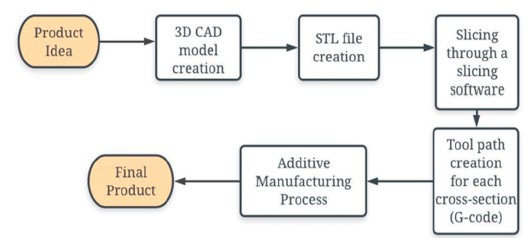
\includegraphics[scale=0.5]{figuras/flujo_trabajo_normal.jpg}
    \caption{Flujo de trabajo convencional \cite{Pinar2019}}
    \label{fig:flujo_trabajo_normal}
\end{figure}

Una parte de la investigación actual del campo de la fabricación aditiva está centrada en la búsqueda de nuevos algoritmos de teselado y \textit{slicing}. Uno de sus objetivos más conocidos la minimización de soportes en voladizo requeridos por figuras complejas \cite{Coupek_2018}, pero también existen otros trabajos enfocados en otros aspectos como la reducción de tiempos de impresión \cite{Karkaria_2024}, el aumento  de propiedades mecánicas \cite{Rosso_2021} o la mejora de acabados finales.

\subsection{Fabricación aditiva robotizada}
El \textit{slicing} uniforme y el adaptativo fueron planteados para sistemas \acrshort{AM} que trabajasen con láminas planas y siempre en la misma dirección. Con el paso del tiempo, se ha podido imprimir cuerpos geométricamente más complejos con la introducción de más grados de libertad. Es decir, se han podido definir una variedad más grande de direcciones de apilamiento de capas y ya no es estrictamente necesario emplear geometrías planas de deposición de material. Esto implica sistemas más precisos y complejos, capaces de asistir en labores de impresión con múltiples direcciones. Es decir, se pasa a emplear manipuladores con configuraciones cinemáticas demás de 3 \acrshort{DOF}, como pueden ser brazos robóticos industriales o de tipo colaborativo entre otros.



\subsubsection*{Tecnologías AM robotizables}
\hypertarget{Tecnologías AM robotizables}{}
\bookmark[level=subsubsection,dest=Tecnologías AM robotizables]{Tecnologías AM robotizables}
Dentro de las diferentes familias de procesos descritas por la norma ISO de fabricación aditiva \cite{ISO-ASTM-52900-2022}, aquellos que pueden integrar fácilmente un manipulador robótico en su flujo de trabajo son los procesos \acrshort{MEX} y \acrshort{DED}. Pese a que existen avances en tecnologías que dispensan gotas de un fotopolímero líquido -como el trabajo de Li et al. \cite{Li_2017}, inspirado en las tecnologías \acrshort{VPP}-  con ayuda de un manipulador robótico, sus aplicaciones por el momento son escasas y se encuentran limitadas a un nicho dentro de aplicaciones biomédicas con hidrogeles específicos. En las siguientes líneas se describirán las dos tecnologías mayoritarias comentando algunas de las aplicaciones más usuales.

\begin{itemize}
    \item \textbf{\acrfull{MEX}}\\
    Es el método más empleado en la fabricación aditiva tradicional. Consiste en una cabeza móvil que toma un filamento de termoplástico y lo funde aportando calor y presión mediante un proceso de extrusión. Algunos de los materiales más empleados son polímeros como el \acrshort{ABS} o el \acrshort{PLA}. No obstante, el ser el método \acrshort{AM} más extendido ha permitido que con el paso del tiempo hayan surgido desarrollos que empleen otros materiales como cera, metales o mezclas de polvos cerámicos \cite{Kruth1998}. También se ha innovado en las técnicas de extrusión de material, de modo que existen equipos que combinan varios extrusores favoreciendo la reducción de costes o el uso conjunto de varios materiales.

    Las piezas resultantes de este proceso se caracterizan por tener un tamaño compacto y por requerir un coste reducido en tareas de acabado y mantenimiento. La figura \ref{fig:zhang_2016_ejemplo_mex_robot} muestra una máquina \acrshort{MEX} robotizada realizada por Zhang et al. \cite{Zhang_2016} En este caso se utilizó un robot ABB  con un extrusor de fabricación propia acoplado (imagen \textit{(a)}) . Para visulizar una imagen previa de la pieza y simular los movimientos del manipulador se utilizó el software de cálculo nativo de ABB (imagen \textit{(b)}. Este ejemplo ha utilizado como material de referencia el \acrshort{ABS} (imagen \textit{(c)}), pero puede extenderse a otros filamentos poliméricos como \acrshort{PLA} o fibras continuas de carbono o vidrio para la producción de composites.

    \begin{figure}[h!]
        \centering
        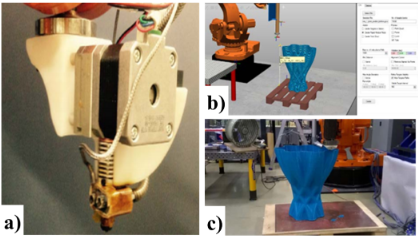
\includegraphics[scale=0.4]{figuras/zhang_2016_ejemplo_mex_robot.png}
        \caption{Estación \acrshort{MEX} robotizada \cite{Zhang_2016}}
        \label{fig:zhang_2016_ejemplo_mex_robot}
    \end{figure}

    \item \textbf{\acrfull{DED}}\\
    Este método emplea una fuente de calor para fundir el material de fabricación mientras se va depositando sobre la superficie de impresión. En concreto, el término hace referencia a que la fuente de energía (láser, haz de electrones o arco de plasma entre otros) tiene el objetivo de derretir un filamento sólido de material para que caiga de forma controlada sobre la cama de impresión. Este proceso se caracteriza por ser el único con capacidad para procesar componentes metálicos, bien sea en forma de polvo o de filamento. Algunas de las aplicaciones de este proceso son la elaboración de geometrías complejas con aleaciones de alta densidad \cite{Caiazzo_2018} o la creación de recubrimientos multimaterial con resistencia a altas temperaturas y la abrasión química \cite{Fujishima_2017}. 

    Estos sistemas presentan ciertas limitaciones en cuanto al elevado número de parámetros de control (potencia del láser, velocidad de alimentación de material, distancia de trabajo, propiedades del material, ángulo de deposición del material, etc.) o la construcción de formas complejas. A causa de estas limitaciones, existe un amplio campo de investigación para optimizar esta tecnología. El trabajo de Ding et al. \cite{Ding_2016} está enfocado en integrar un sistema de deposición láser móvil con una plataforma móvil para reorientar paulatinamente la pieza resultado según se fabrica (Figura \ref{fig:ejemplo_ding_2016}). Por su parte, empresas como Meltio \cite{Meltio_web} son especialistas en deposición por arco de plasma y su integración con sistemas robotizados ya existentes, como puede verse en la Figura \ref{fig:ejemplo_meltio}.

    \begin{figure}[h!]
        \centering
         \begin{subfigure}[h]{0.45\linewidth} 
            \centering
            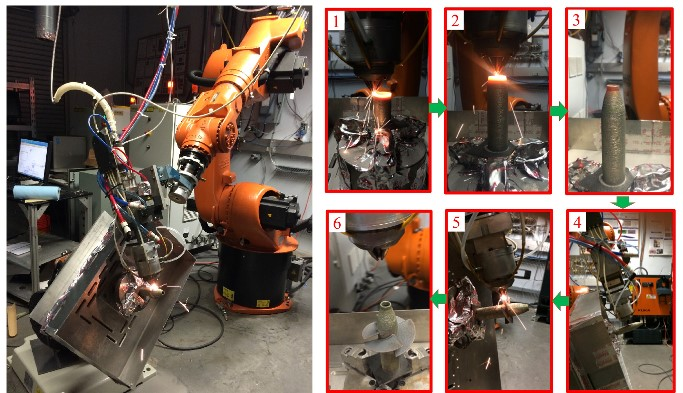
\includegraphics[scale=0.35]{figuras/ejemplo_ding_2016.jpg}
            \caption{Deposición láser móvil robotizada \cite{Ding_2016}}
            \label{fig:ejemplo_ding_2016}
        \end{subfigure}
        \begin{subfigure}[h]{0.45\linewidth} 
            \centering
            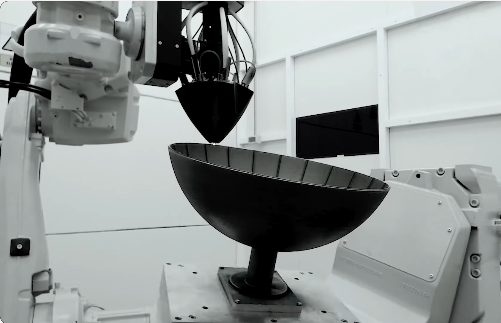
\includegraphics[scale=0.45]{figuras/ejemplo_meltio.png}
            \caption{Arco de plasma robotizado \cite{Meltio_web}.}
            \label{fig:ejemplo_meltio}
        \end{subfigure}
        \caption{Procesos \acrshort{DED}}
    \end{figure}

    
\end{itemize}
 
Cuando se pretende emplear un brazo robótico en el proceso de fabricación aditiva, la literatura tiende a referirse a él como un proceso de \textit{Impresión con manipuladores de más de 3 \acrshort{DOF}}. El brazo robótico puede modificar con gran precisión la trayectoria y velocidad de deposición del material. El manipulador puede operar directamente el extrusor o la cama de impresión, lo cual le dota de una gran libertad de movimiento para conseguir diseños no planares. Este es el modelo de impresión \acrshort{NPAM} utilizado en este trabajo. La figura \ref{fig:impresion_3d_robotica} es un ejemplo de una estación con 8 \acrshort{DOF}, donde 6 corresponden al robot y 2 a la cama de impresión móvil.

\begin{figure}[h!]
    \centering
    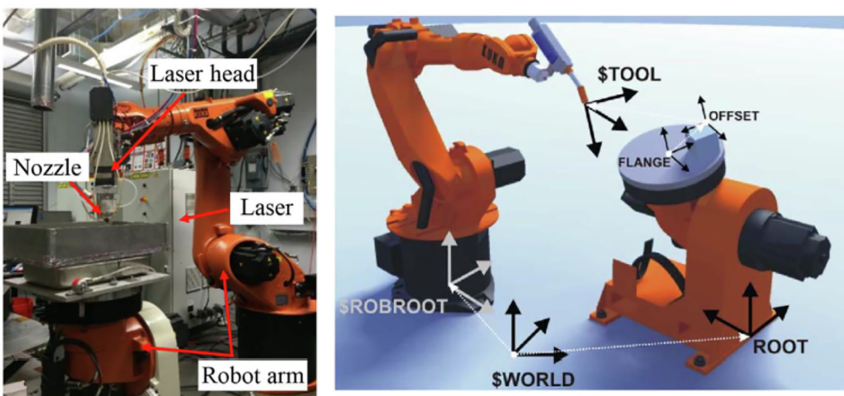
\includegraphics[scale=0.3]{figuras/impresion_3d_robotica.png}
    \caption{Impresión robótica con 8 \acrshort{DOF} \cite{Shah_2022}}
    \label{fig:impresion_3d_robotica}
\end{figure}

\subsubsection*{Preparación del manipulador}
\hypertarget{Preparación del manipulador}{}
\bookmark[level=subsubsection,dest=Preparación del manipulador]{Preparación del manipulador}

La literatura establece que los procesos de fabricación pueden transcurrir cíclicamente a lo largo de un intervalo de tiempo conocido como tiempo de ciclo \cite{Kalpajkin_2006}. El tiempo de ciclo puede establecerse como la sucesión de cuatro etapas directamente relacionadas con la manipulación de materia prima y la elaboración del producto industrial: espera, preparación, operación y post-procesado.

La figura \ref{fig:tiempo_ciclo} muestra un esquema de cómo se suceden estas etapas durante el tiempo de ciclo del proceso. Nótese que en los extremos de esta sucesión también se define una cantidad de tiempo variable correspondiente al transporte de información, materiales, equipos y mano de obra entre procesos.

\begin{figure}[h!]
    \centering
    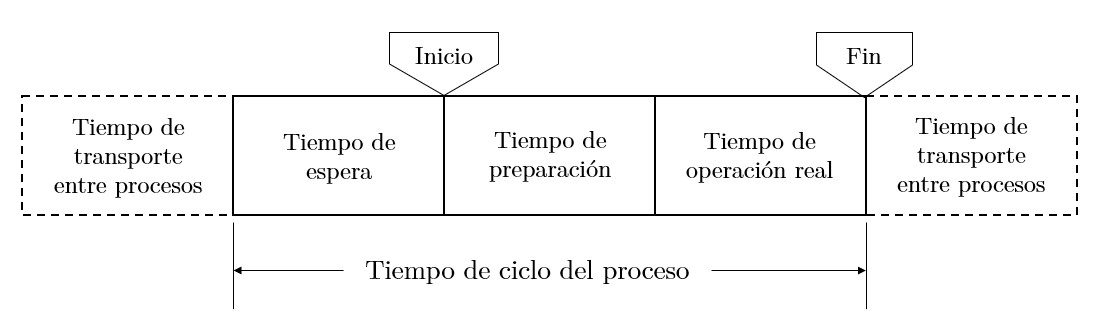
\includegraphics[scale=0.4]{figuras/tiempo_ciclo_v2.jpg}
    \caption{Etapas del tiempo de ciclo \cite{Kalpajkin_2006}}
    \label{fig:tiempo_ciclo}
\end{figure}

Un proceso de fabricación aditiva robotizada también sigue esta estructura. La etapa de preparación, en concreto, es de vital importancia para calibrar con antelación todos los sistemas que participarán en el proceso. Independientemente del elemento móvil que se desee integrar con el robot, siempre es necesario implementar una serie de sistemas que permitan calcular una trayectoria que debe seguir el manipulador y que puedan compensar las inercias y desplazamientos no deseados del robot. Para ello se establece un procedimiento durante la etapa de preparación denominado \textit{calibración} en el que se define la posición del manipulador en el espacio de trabajo y se estudia el trazado de trayectorias simples, así como también en otros sistemas de referencia asociados a un sistema global.

Durante la calibración es posible extraer los factores que pueden intervenir en el desvío existente entre la trayectoria que se proyecta en el diseño \acrshort{CAD} de la pieza, la calculada por el software del manipulador y la efectuada por manipulador en sí. La calibración puede ser de dos tipos diferentes:

\begin{itemize}
    \item \textbf{Calibración extrínseca:} Centrada en determinar las relaciones existentes entre los sistemas de coordenadas empleados por el robot y su entorno exterior que lo rodea. Algunos de los métodos de calibración extrínseca que han tenido mejores resultados son los propuestos por Kato et al. \cite{Kato_2021}, que se basa en el uso de un algoritmo de árbol de decisión para corregir la desviación existente entre la pose cartesiana calculada y la alcanzada en la realidad; Zheng et al. \cite{Zheng_2022}, que implementa algoritmos genéticos para corregir las funciones objetivo que minimicen la desviación de las posiciones tras varias iteraciones consecutivas; o por Guzmán et al.\cite{Guzman_2023} que propone un flujo de trabajo generalizado adaptable a varias estaciones y fundamentado en obtener la calibración de zonas clave de la estación de trabajo e ir relacionándolas de forma sucesiva con unos utillajes diseñados especialmente para dicha función.

    \item \textbf{Calibración intrínseca:} Enfocada en determinar aquellos parámetros geométricos, dinámicos, eléctricos y de control del propio robot que pueden influir en su comportamiento. Métodos de este tipo de calibración notables son los aportados por Nubiola et al.\cite{Nubiola2013}, que analiza las inercias asociadas a cada eslabón y articulación de un robot manipulador y propone una serie de funciones que minimizan los errores de cálculo de coordenadas articulares en la fase de cálculo de trayectoria software del robot; el trabajo de Moller et al.\cite{Moller_2017} enfocado en establecer un bucle de control con los encoders de cada articulación para reducir su inercia de giro y poder corregir las diferentes posiciones calculadas de forma previa a la ejecución; o el definido por Villagrossi et al.\cite{Villagrossi2018} que entrelaza tres bucles de control enfocados en modificar en tiempo real la alimentación de material, el ángulo de ataque adoptado por la herramienta y la fuerza final ejercida por el manipulador.
\end{itemize}

\subsubsection*{Sistemas de referencia y métodos de aprendizaje}
\hypertarget{Sistemas de referencia y métodos de aprendizaje}{}
\bookmark[level=subsubsection,dest=Sistemas de referencia y métodos de aprendizaje]{Sistemas de referencia y métodos de aprendizaje}

En cualquier proceso de fabricación robótica siempre será necesario disponer de al menos tres sistemas de referencia (Figura \ref{fig:Robotics-coordinate-systems}). Estos sistemas deben relacionarse entre sí para definir el proceso de fabricación. Estos son: (1) sistema de referencia de la máquina, (2) sistema de referencia de la pieza y (3) sistema de referencia de la herramienta.

Dependiendo de la aplicación, se pueden añadir más sistemas de referencia y enlazarlos mutuamente. No obstante, se debe tener en cuenta que los sistemas de referencia disponibles deben relacionarse a través de una serie de transformaciones matriciales que permitan definir de forma unívoca el movimiento del robot.
    
\begin{figure}[h!]
    \centering
    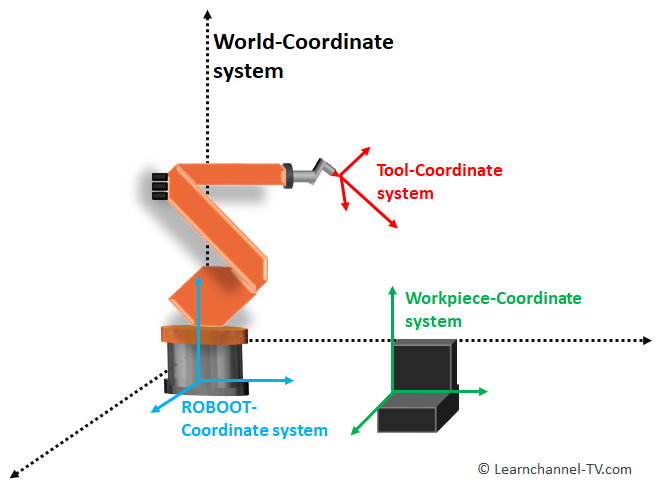
\includegraphics[scale=0.4]{figuras/Robotics-coordinate-systems.png}
    \caption{Sistemas de coordenadas de un robot \cite{Robot_Coordinate_Systems}}
    \label{fig:Robotics-coordinate-systems}
\end{figure}

La trayectoria puede obtenerse a gracias a los \textit{métodos de aprendizaje}, un conjunto de operaciones que permite al robot y su controlador calcular los puntos de la trayectoria y definir los pares y velocidades necesarios para llevarla a cabo. Los métodos de aprendizaje pueden clasificarse como:
\begin{itemize}
    \item \textbf{Aprendizaje \textit{online} o in-situ:} Se despalaza el robot manualmente a los puntos deseados de la trayectoria para registrarlos uno a uno e implementar un controlador especialmente definido para ese movimiento. Pese a que este tipo de aprendizaje aporta una precisión del orden de la repetibilidad\footnote{Capacidad de un mecanismo automático para retornar a la posición inicial varias veces siempre bajo las mismas condiciones} de la unidad empleada, sus mayores inconvenientes son que requiere de un tiempo elevado de preparación y debe repetirse la operación cada vez que se haga una nueva configuración a la estación. 
    \item \textbf{Aprendizaje \textit{offline} o planificado:} La trayectoria se plantea de forma teórica gracias a diferentes aplicaciones software y se traslada a un código ejecutable por el robot físico \cite{Botazzi_2005}. Estos métodos de aprendizaje necesitan usualmente de un marco de referencia que represente su entorno real. Las soluciones más empleados habitualmente son integrar un modelo \acrshort{CAD} en el espacio de trabajo virtual \cite{Botazzi_2006} o reconstruir el objeto real a partir de sistemas de visión por computador \cite{Liu_2010}.
    \item \textbf{Aprendizaje híbrido:} Este método emplea un flujo de trabajo basado en una combinación de los dos anteriores. En una primera fase se define una trayectoria concreta y se indica al robot cómo alcanzar el primer punto mediante un proceso de aprendizaje online. Cuando el robot ha podido desplazarse desde su pose original a la pose comienzo de la trayectoria objetivo, se inicia inmediatamente una segunda fase de aprendizaje offline en la que se calcula el trazado del resto de puntos de la trayectoria. Uno de los usos con más potencial de estos sistemas de aprendizaje es la corrección dinámica -mientras se efectúa el proceso de fabricación- de desviaciones existentes entre la pieza real y el modelo \acrshort{CAD} \cite{Zheng_2022}.
\end{itemize}
    
Una representación simple de los métodos de aprendizaje online y offline puede verse en la Figura \ref{fig:aprendizaje_online_offline}. En los años recientes, el aprendizaje offline está cobrando una relevancia especial de cara a los procesos robotizados gracias a la mayor versatilidad que aporta en el cálculo y trazado de trayectorias, que pasa a ser responsabilidad de una capa de software especializado. Las técnicas de aprendizaje offline en muchas ocasiones necesitan acompañarse de técnicas de calibración extrínseca de alta fiabilidad para garantizar la ejecución de la trayectoria calculada y también la integridad del equipo empleado junto a sus usuarios.

\begin{figure}[h!]
    \centering
    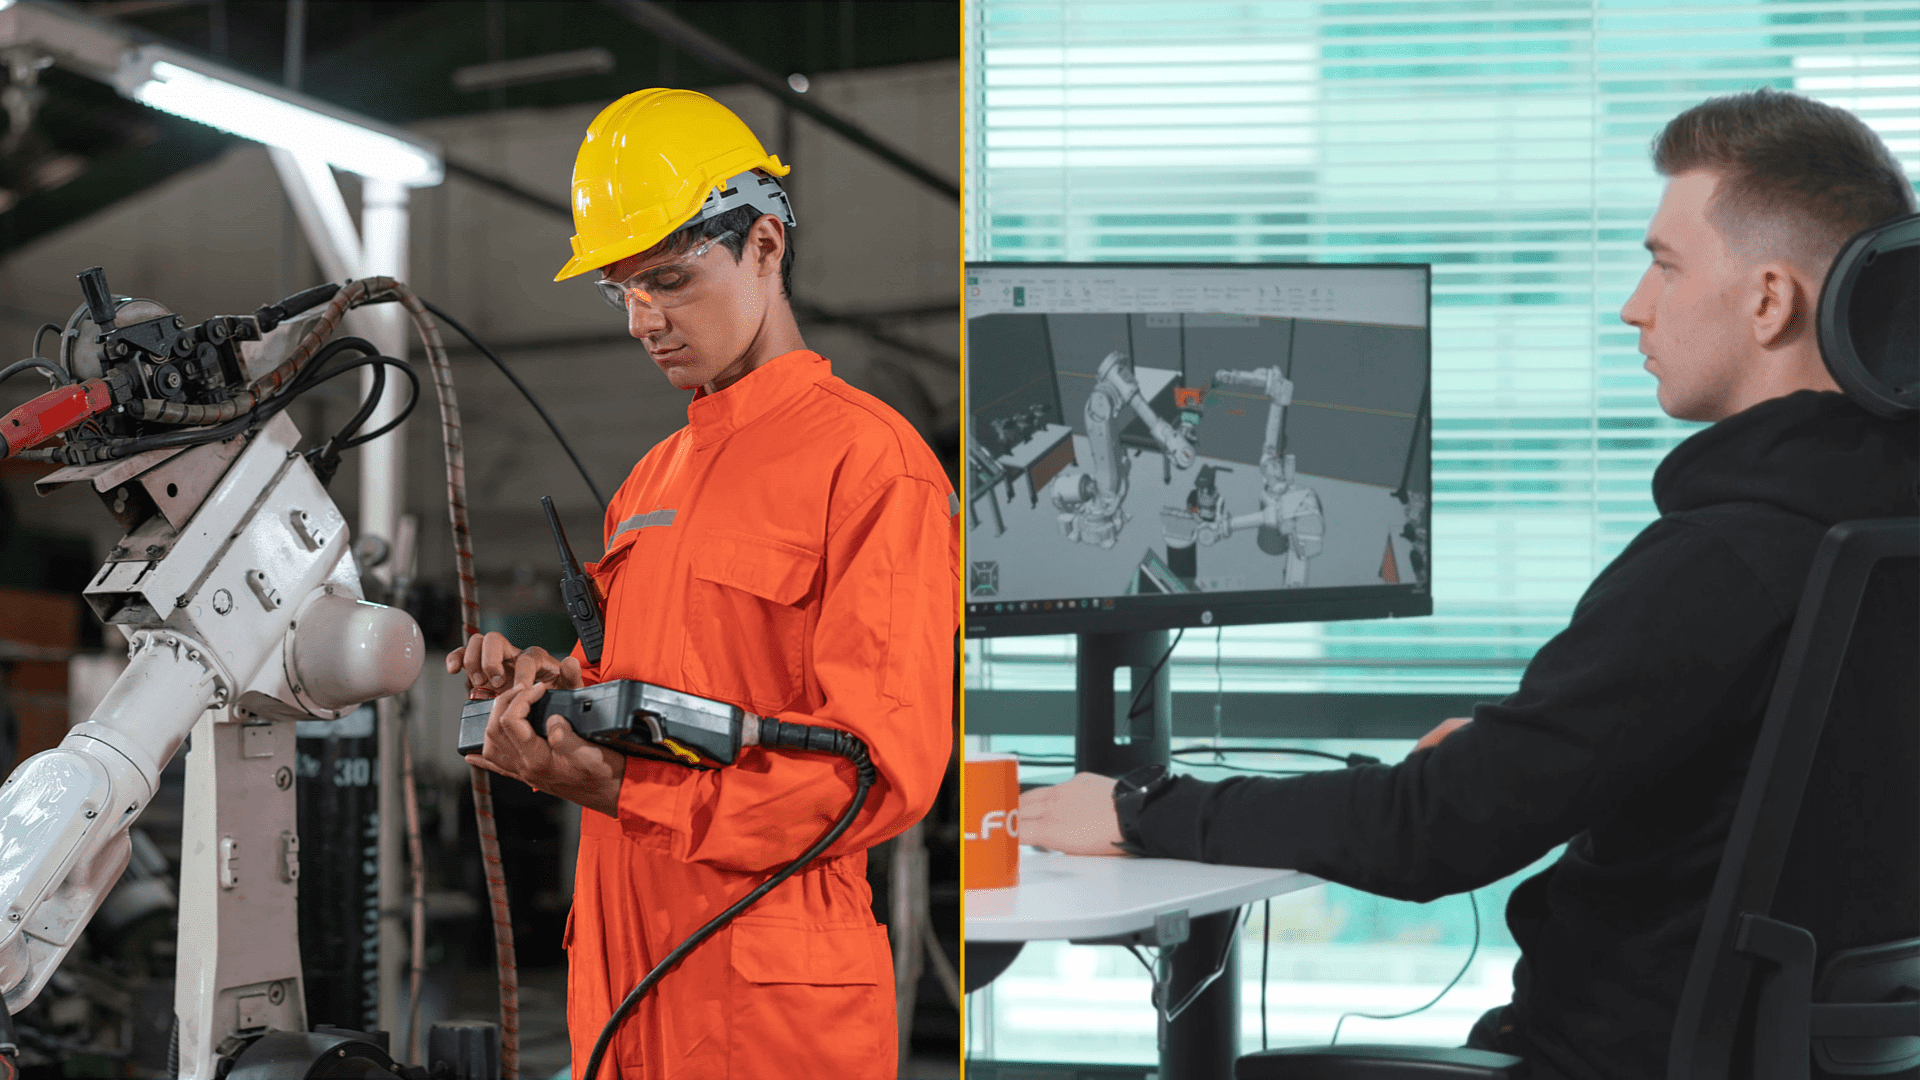
\includegraphics[scale=0.15]{figuras/aprendizaje_online_offline.png}
    \caption{Ejemplo de aprendizaje online (izquierda) y offline (derecha)}
    \label{fig:aprendizaje_online_offline}
\end{figure}

\subsubsection*{Arquitecturas informáticas}
\hypertarget{Arquitecturas informáticas}{}
\bookmark[level=subsubsection,dest=Arquitecturas informáticas]{Arquitecturas informáticas}
\label{sec: arquitecturas_informaticas_estado_arte}

Las tareas antes vistas suponen operaciones matemáticamente complejas que deben realizarse con ayuda de un equipo software especializado. Por otro lado, el brazo robótico debe poder comunicarse con otros elementos de su espacio de trabajo para disponer de información constante acerca de parámetros cinemáticos (posición, velocidad y aceleración), dinámicos (fuerzas y torques articulares), materiales (temperatura, presión y flujo) o mandatos del operario humano. 

El manipulador robótico por sí solo no es suficiente para gestionar todo este volumen de información y necesita de elementos auxiliares. Es decir, el brazo robótico debe formar parte de una arquitectura de comunicaciones industriales más grande.

Para poder integrar el manipulador robótico en este tipo de arquitecturas, se deben introducir modificaciones al flujo de trabajo explicado en la sección \ref{sec:flujo_trabajo}. La figura \ref{fig:flujo_trabajo_robot} sirve de ejemplo, en este caso se toma el trabajo de un equipo del Virginia Tech con un robot ABB  1200-7 \cite{Kubalak2016}. Su mayor aporte es la introducción de una unidad de control responsable del proceso de \textit{parseo} \footnote{Conjunto de operaciones de lectura de un fichero estandarizado para obtener los parámetros más representativos en un proceso automatizado. En la literatura de la \acrshort{AM} se puede interpretar como la lectura del código \acrshort{AMF} para trazar la trayectoria de los elementos móviles.} a partir del \acrshort{AMF} que además establezca una realimentación interna con las articulaciones del robot para corregir trayectorias.

\begin{figure}[h!]
    \centering
    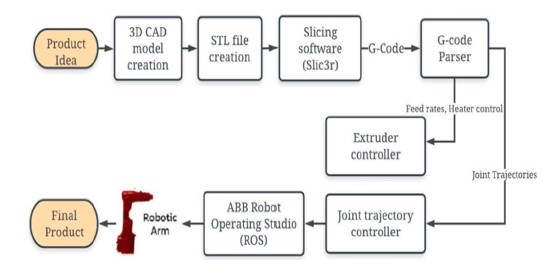
\includegraphics[scale=0.5]{figuras/flujo_trabajo_robot.jpg}
    \caption{Flujo de trabajo con un manipulador robótico incorporado \cite{Kubalak2016}}
    \label{fig:flujo_trabajo_robot}
\end{figure}

Los modelos más básicos se fundamentan en la implementación de una librería de código para el cálculo de trayectorias y el envío de mensajes. Estos modelos ya establecieron los tres agentes fundamentales en este tipo de sistemas: un controlador local para el cálculo de trayectorias, otro específico para el manipulador robótico y una interfaz que adaptase los mensajes entre ambos.

Uno de los sistemas más detallados fue el propuesto por Huang et al. \cite{Huang_2003}, mostrado en la Figura \ref{fig:modelo_arquitectura_antiguo}. Este sistema se caracteriza por establecer un modelo sencillo y robusto que además incorporaba una nueva capa de control supervisado por computador. El trabajo de Santos et al. \cite{Santos_2005} estaba más enfocado en un desarrollo de software portable y fácil de programar con varios lenguajes. No obstante ya propuso utilizar en desarrollos futuros comunicaciones industriales (protocolo Ethernet en concreto) para introducir una capa de procesamiento de datos distribuida, como puede verse en la Figura \ref{fig:arquitectura_ethernet}.

    \begin{figure}[h!]
        \centering
         \begin{subfigure}[h]{0.45\linewidth} 
            \centering
            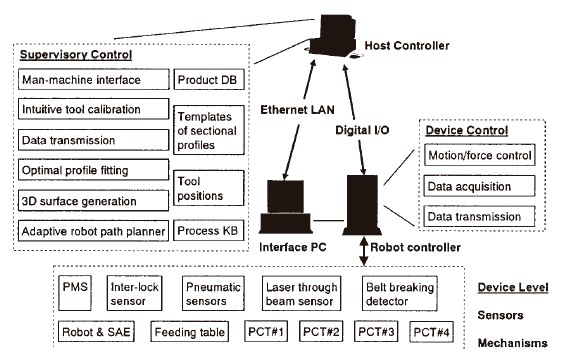
\includegraphics[scale=0.50]{figuras/modelo_arquitectura_antiguo.jpg}
            \caption{Modelo de tres agentes \cite{Huang_2003}}
            \label{fig:modelo_arquitectura_antiguo}
        \end{subfigure}
        \begin{subfigure}[h]{0.45\linewidth} 
            \centering
            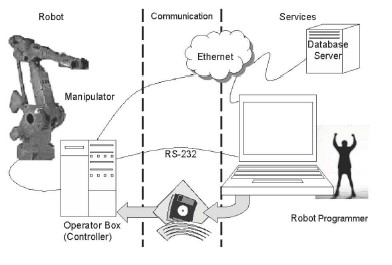
\includegraphics[scale=0.65]{figuras/arquitectura_ethernet.jpg}
            \caption{Comunicaciones por Ethernet \cite{Santos_2005}}
            \label{fig:arquitectura_ethernet}
        \end{subfigure}
        \caption{Primeras arquitecturas informáticas}
    \end{figure}

El paso del tiempo y el desarrollo de la microelectrónica favoreció la introducción de los sensores y actuadores con los que cuentan los robots industriales hoy en día. Con estos dispositivos se ha podido desarrollar modificaciones más especializadas de los primeros modelos de arquitectura informática, especialmente en el campo de la calibración y aprendizaje del robot.  

Del lado de la calibración se tiene parte del trabajo de Villagrossi et al. \cite{Villagrossi2018}. La Figura \ref{fig:arqutiectura_control_villagrossi} muestra cómo toma un ordenador industrial para implementar su triple bucle de control y se sirve de una capa de comunicaciones por protocolo \acrshort{TCP/IP} para enviar las acciones correctoras a un controlador diseñado específicamente para el robot. Como muestra la Figura \ref{fig:arquitectura_zheng_capas}, la propuesta de Zheng et al. \cite{Zheng_2022} se caracteriza por establecer cuatro capas de software especializadas en la interacción con el operador humano, el análisis de datos, la programación de movimientos y una interfaz de comunicaciones con ayuda del \acrshort{PLC} del robot.

    \begin{figure}[h!]
        \centering
         \begin{subfigure}[h]{0.45\linewidth} 
            \centering
            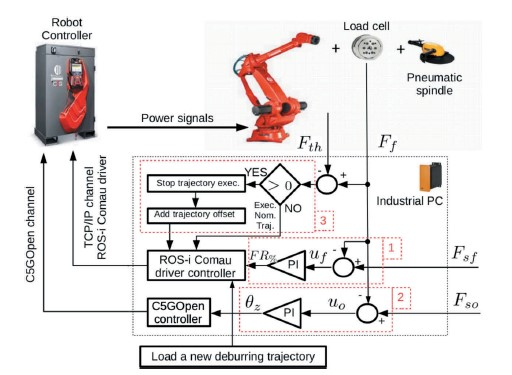
\includegraphics[scale=0.35]{figuras/arqutiectura_control_villagrossi.jpg}
            \caption{Ordenador y comunicaciones \acrshort{TCP/IP} \cite{Villagrossi2018}}
            \label{fig:arqutiectura_control_villagrossi}
        \end{subfigure}
        \begin{subfigure}[h]{0.45\linewidth} 
            \centering
            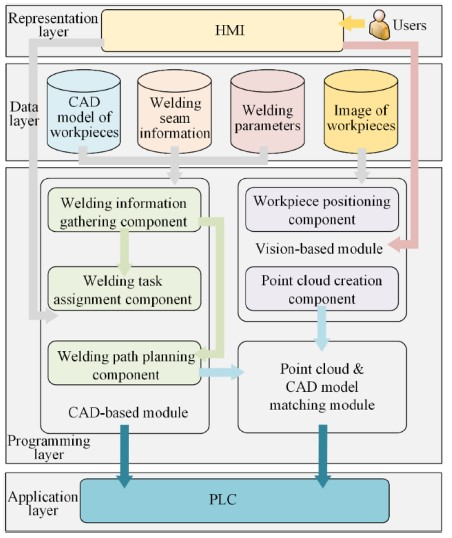
\includegraphics[scale=0.25]{figuras/arquitectura_zheng_capas.jpg}
            \caption{Capas especializadas de software \cite{Zheng_2022}}
            \label{fig:arquitectura_zheng_capas}
        \end{subfigure}
        \caption{Arquitecturas especializadas en calibración}
    \end{figure}

Por su parte, el aprendizaje también representa desarrollos interesantes en arquitecturas de estaciones robotizadas, especialmente el de tipo offline. Este tipo de arquitecturas se ven reforzadas por el uso de entornos de programación robótica como puede ser el caso de \acrshort{ROS}. 

El trabajo de Wei et al.\cite{Wei_2018} expone un diseño de arquitectura que minimiza la programación directa entre hombre y máquina. Este modelo se muestra en la Figura \ref{fig:arquitectura_Wei_2018} en forma de flujo de trabajo con capas de diferente nivel de abstracción. Se caracteriza por ser compatible con sistemas operativos de uso general y el uso de programación con \acrshort{ROS} para definir unos bloques de funciones específicas (como puede ser el control de un AGV, detección de humanos en el entorno o un generador de trayectorias de mecanizado a partir de un modelo \acrshort{CAD}). Los bloques función cuentan con su propia interfaz, por lo que una de las limitaciones que se trató de solventar fue la definición de unas capas intermedias de mensajes.

\begin{figure}[h!]
    \centering
    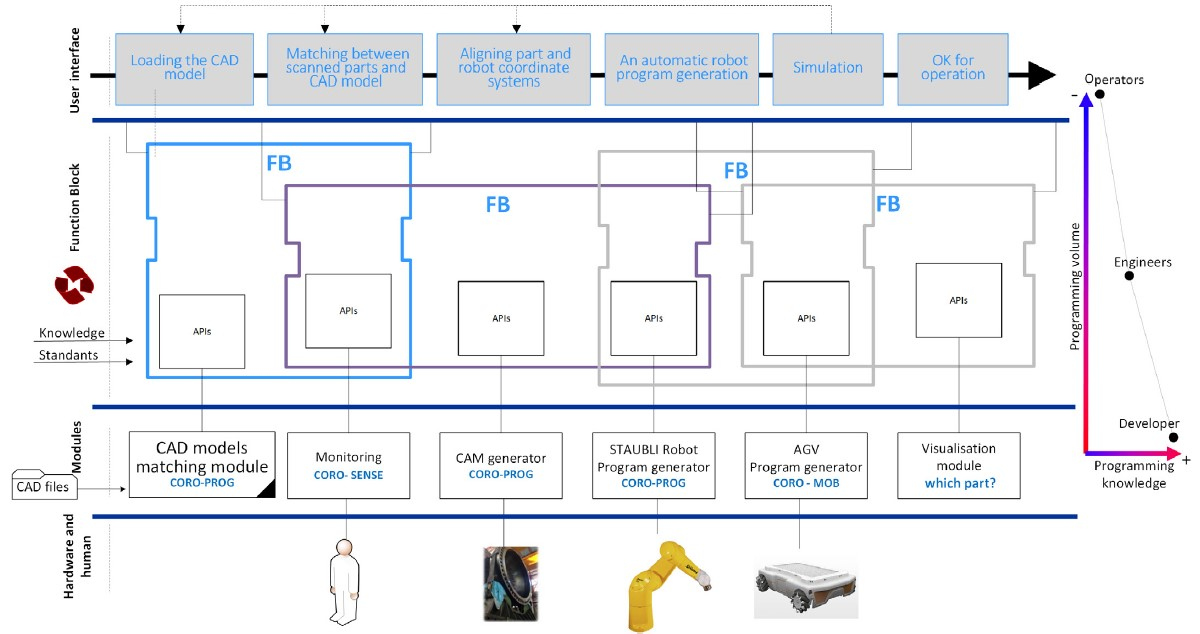
\includegraphics[scale=0.35]{figuras/arquitectura_Wei_2018.jpg}
    \caption{Flujo de trabajo y arquitectura por capas de \acrshort{ROS} especializadas \cite{Wei_2018}}
    \label{fig:arquitectura_Wei_2018}
\end{figure}

Otra de las grandes limitaciones en las arquitecturas informáticas enfocadas en el aprendizaje online son los métodos de comprobación de las trayectorias generadas. Verl et al. \cite{Verl_2019} expone en su revisión que muchos sistemas que basan su cálculo de trayectorias en modelos de inteligencia artificial que minimizan un parámetro de error. Como puede observarse en el procedimiento representado por la Figura \ref{fig:correccion_trayectorias_offline}, la compensación de errores suele darse en la etapa de cálculo de trayectoria o justo antes de enviarla al manipulador robótico, a modo de revisión previa. En otras palabras, a priori no existe un método definido para comprobar la exactitud durante la fabricación del resultado final y se deja a la propia pericia y experiencia del operario.

\begin{figure}[h!]
    \centering
    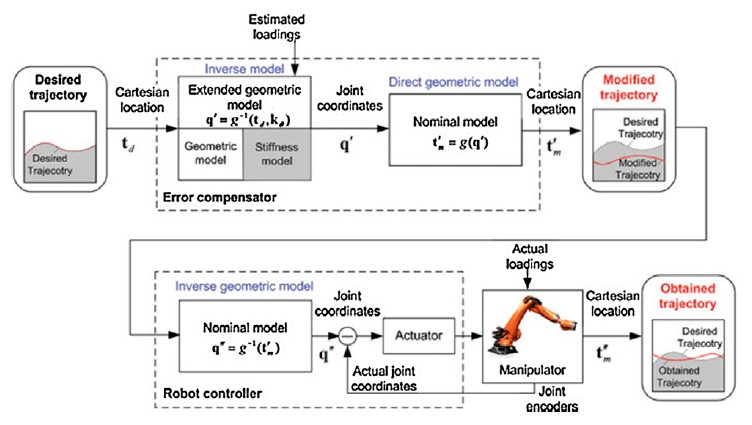
\includegraphics[scale=0.5]{figuras/correccion_trayectorias_offline.jpg}
    \caption{Corrección offline de trayectorias \cite{Klimchik2014}}
    \label{fig:correccion_trayectorias_offline}
\end{figure}

Cada vez más arquitecturas informáticas de este tipo integran sistemas de corrección de trayectoria durante la ejecución, para minimizar los errores del producto final. Esta solución necesita que la estación se adapte rápidamente a las necesidades de fabricación, por lo que se recurre a soluciones basadas en bloques de control individuales que se comunican entre sí. La Figura \ref{fig:arquitectura_controlador_celda} es un ejemplo de este paradigma. En ella se establecen varios bloques función con su propia programación y algoritmos de control, no obstante todos ellos se comunican entre sí a través de una interfaz de mensajes común. Esta interfaz es la definida por un elemento central que hace de controlador general de la estación (en color salmón en la Figura \ref{fig:arquitectura_controlador_celda}).

\begin{figure}[h!]
    \centering
    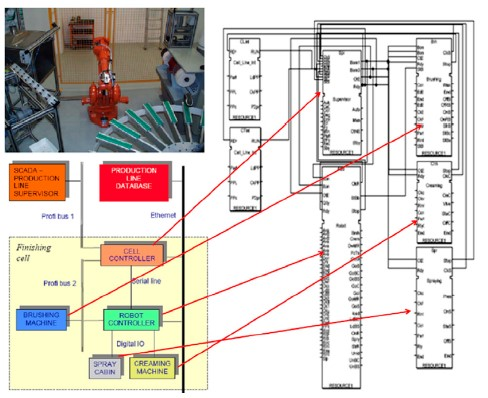
\includegraphics[scale=0.5]{figuras/arquitectura_controlador_celda.jpg}
    \caption{Arquitectura con controlador central de celda \cite{Verl_2019}}
    \label{fig:arquitectura_controlador_celda}
\end{figure}


\subsection{Fabricación aditiva no planar (\acrshort{NPAM})}
La implementación de dispositivos robóticos con más de tres \acrshort{DOF} en procesos de fabricación aditiva  supone una mayor libertad en el diseño y desarrollo de nuevas geometrías. Este enfoque se ve favorecido gracias a que un mayor número de grados de libertad permite configuraciones cinemáticas más complejas, pudiendo llegar a puntos que con otras tecnologías estaban restringidos para el equipo de diseño de la pieza. El manipulador robótico y los equipos hardware anexos pueden asumir la responsabilidad de calcular nuevas trayectorias y movimientos de deposición de forma independiente y modular.

Es decir, el proceso incrementa su eficiencia y se abre la puerta a que se aborden nuevas geometrías que puedan optimizar otros aspectos del proceso de fabricación como pueden ser configuraciones geométricas, empleo de material, uso de soportes de impresión o mejora de las propiedades mecánicas. Un ejemplo de aplicación directa de este enfoque son los procesos de fabricación \acrshort{NPAM}

La \acrshort{NPAM} es una técnica avanzada de fabricación aditiva que se caracteriza por permitir la impresión de geometrías de capa con curvatura. Es decir, las piezas resultantes de este proceso no se ven sometidas a las restricciones típicas de la \acrshort{AM} basada en la deposición de material en capas planas horizontales, como son:

\begin{itemize}
    \item \textbf{Direcciones privilegiadas:} Los elementos fabricados mediante impresión 3D tradicional se han realizado mediante la acumulación de capas planas. Esta disposición favorece un comportamiento anisótropo muy restringido, esto es, existen direcciones muy claras en las que el producto final es más resistente ante un esfuerzo concreto que otras. En el caso de la fabricación aditiva mediante capas planas convencionales, estas direcciones suelen ser trazados rectos y paralelos al plano de impresión.
    
    \item \textbf{Adhesión entre capas:} En los procesos \acrshort{AM} siempre se busca obtener un resultado final lo más macizo posible. Esto implica que las capas de deposición deben evitar el deslizamiento entre ellas, ya que puede afectar a la rugosidad, acabados y comportamiento mecánico de la pieza. Nótese en la figura \ref{fig:comportamiento_anisotropo3} cómo la deposición en capas poco adheridas favorece una anisotropía de la pieza en la dirección longitudinal, es decir, la perpendicular a las capas.

    \item \textbf{Movimiento tridimensional:} Las técnicas \acrshort{AM} tradicionales solamente pueden desplazarse en movimientos que resulten de una combinación de las direcciones cartesianas XYZ. Por otro lado, las piezas diseñadas y enviadas a imprimir cuentan siempre con partes con una parametrización cartesiana compleja que obliga a emplear soportes cuando existen voladizos. Un ejemplo puede verse en la figura \ref{fig:fdm_soporte_desventaja}.
\end{itemize}

   \begin{figure}[h!]
        \begin{subfigure}[h!]{0.45\linewidth} 
            \centering
            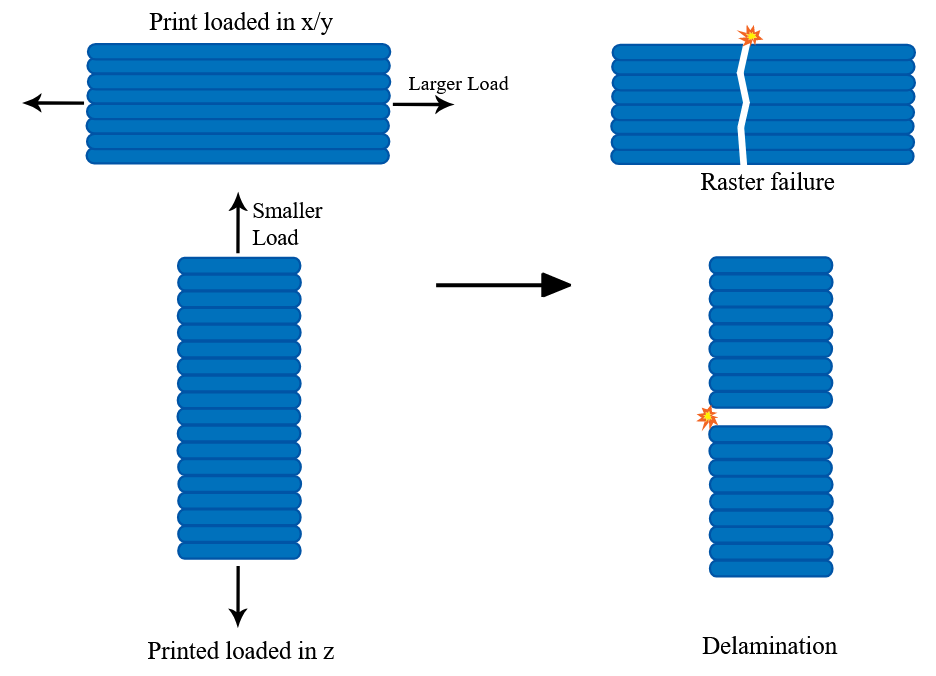
\includegraphics[scale=0.25]{figuras/comportamiento_anisotropo3.png}
            \caption{Comportamiento anisótropo entre capas\cite{web_fdm_properties}}
            \label{fig:comportamiento_anisotropo3}
        \end{subfigure}
        \begin{subfigure}[h!]{0.45\linewidth} 
            \centering
            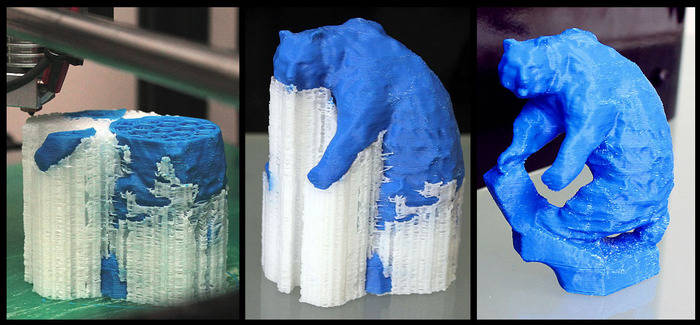
\includegraphics[scale=0.25]{figuras/fdm_soporte_desventaja.jpg}
            \caption{Uso de soportes para piezas con voladizos}
            \label{fig:fdm_soporte_desventaja}
        \end{subfigure}
        \caption{Limitaciones de la \acrshort{AM} tradicional}
    \end{figure}

La \acrshort{NPAM} solventa estas problemáticas y supone ventajas como:
\begin{itemize}
    \item \textbf{Complejidad geométrica:} Se puede imprimir sobre capas con curvatura directamente. De este modo se pueden conseguir buenos resultados en figuras basadas en estructuras curvas o con una gran cantidad de voladizos, cosa que en modelos más tradicionales de fabricación aditiva resultaría imposible.

    \item \textbf{Mayor capacidad de personalización:} Se pueden trazar trayectorias curvas más complejas, este aspecto puede ser de gran utilidad para la fabricación de dispositivos para necesidades específicas. Como ejemplo, en la figura \ref{fig: am_geometria_anatomica} se muestra cómo se utiliza un proceso de este tipo para poder imprimir capas de tejido sobre modelos biológicos.
    
     \begin{figure}[h!]
         \centering
         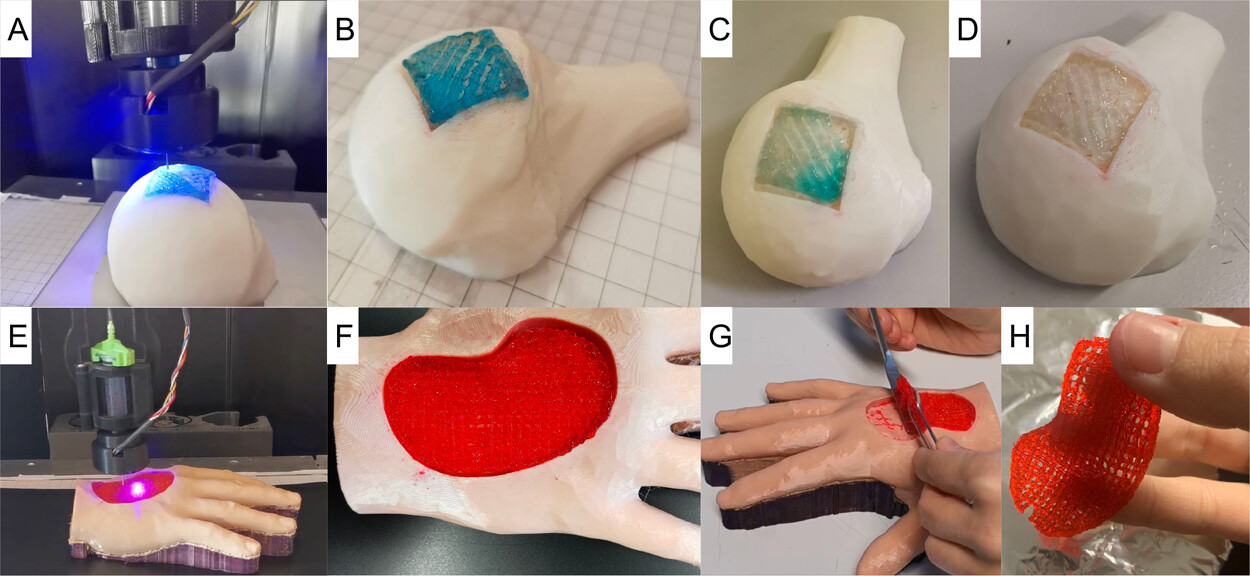
\includegraphics[scale=0.5]{figuras/am_geometria_anatomica.jpeg}
         \caption{Impresión \acrshort{NPAM} sobre modelos humanos \cite{Fortunato_2023}}
         \label{fig: am_geometria_anatomica}
     \end{figure}

    \item \textbf{Mejora de propiedades mecánicas:} La posibilidad de seleccionar impresiones en multitud de direcciones y tipos de capas permite reducir la anisotropía del resultado final, aumentando su resistencia a tracción y fatiga. En otras palabras, se orienta la dirección de anisotropía de forma favorable a los casos de carga en servicio de la pieza deseada. La figura \ref{fig:am_ensayos_resistencia_npam} muestra la comparativa entre una pieza modelo impresa por capas planas y otra mediante capas curvas.

    \begin{figure}[h!]
        \centering
        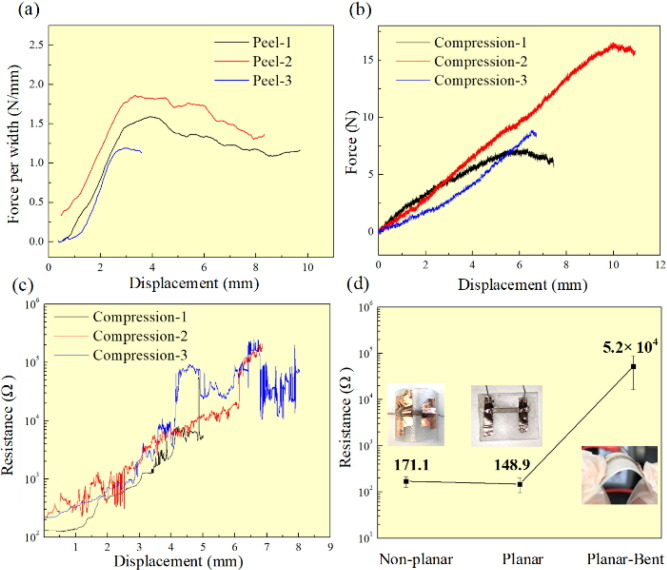
\includegraphics[scale=0.3]{figuras/am_ensayos_resistencia_npam.jpg}
        \caption{Mejora de propiedades mecánicas en productos NPAM \cite{Jiang_2021}}
        \label{fig:am_ensayos_resistencia_npam}
    \end{figure}

    \item \textbf{Eficiencia aumentada:} La \acrshort{NPAM} no solamente aporta resultados más personalizados y con propiedades mecánicas superiores, si no que también es efectiva para la introducción de economías de escala en grandes cantidades de piezas. Todo a causa de que se reduce la impresión de voladizos, se favorece el reciclaje de los soportes de impresión y se ahorra material. Este enfoque resulta altamente provechoso ya no solo desde una perspectiva económica, si no también desde una medioambiental \cite{Cendrero_2021}.
\end{itemize}

\section{Limitaciones y motivación}
En esta sección se definen las limitaciones del estado de la ciencia hasta el momento, indicando aquellos que pueden resultar de mayor interés de cara a efectuar una aplicación industrial práctica y adaptable al entorno de trabajo. En una segunda parte, se definirán las limitaciones de mayor impacto y que sirven también de motivación para el proyecto final.

\subsection{Limitaciones} \label{seccion: Limitaciones}
El presente proyecto trabaja con un robot colaborativo que sirve como herramienta principal de una estación \acrshort{NPAM}. A diferencia de muchos ejemplos observados en la literatura -que se basan en utilizar una boquilla extrusora móvil integrada con el cabezal del robot- aquí se plantea restringir los grados de libertad asociados a la boquilla extrusora en pro del desplazamiento de la cama de impresión. 

\subsubsection*{Arquitecturas de estación}
\hypertarget{Arquitecturas de estación}{}
\bookmark[level=subsubsection,dest=Arquitecturas de estación]{Arquitecturas de estación}

Las arquitecturas informáticas de estaciones robotizadas deben ser capaces de realizar varias tareas complejas como son el cálculo de trayectoria, la compensación de errores, la toma de datos en directo o la gestión de información en tiempo real. Por lo que las soluciones suelen tender hacia modelos compuestos por varios controladores especializados. Cada controlador deberá comunicarse con los demás a través de una serie de mensajes comunes bien entre una pareja específica o con ayuda de un bloque global de gestión.

No existe un modelo único, si no que se establece a partir de una base y trata de adaptarse a las necesidades de fabricación aditiva. En concreto, en el caso de aquellas estaciones que incorporan elementos de fabricación \acrshort{NPAM} cobran una especial relevancia las tareas de cálculo de desplazamientos y corrección de trayectorias, paro los que se prefiere introducir su propio esquema de comunicaciones.

Sin embargo, una arquitectura de comunicaciones no puede limitarse a optimizar las tareas más relevantes dentro de cada proceso, si no que también debe crear un entorno común al resto de agentes que la integran. Es decir, se debe disponer de un controlador que pueda gestionar toda esta información.

El paso del tiempo ha hecho que se definan lenguajes que sirven para diseñar mensajes de diferentes tipos, pero todavía queda en responsabilidad del ingeniero definir la información más relevante y cómo ha de tratarse.


\subsubsection*{Entorno de trabajo}
\hypertarget{Entorno de trabajo}{}
\bookmark[level=subsubsection,dest=Entorno de trabajo]{Entorno de trabajo}

Para llevar las operaciones de calibración y aprendizaje, los robots comerciales suelen implementar su propia solución en forma de entorno de trabajo o \textit{framework}. De cara a la operación del robot, esta estrategia supone ventajas como reducir de la curva de aprendizaje del manejo del equipo, acelerar la puesta en marcha de proyectos o aprovechar al máximo el hardware del equipo. De cara a aplicaciones que requieren de una mayor flexibilidad, esta dependencia del entorno del fabricante puede dificultar la integración del manipulador con otros sistemas y componentes externos, limitar la portabilidad y escalado del código o reducir la vida útil del equipo a unas aplicaciones muy concretas.

Ante estos desafíos, en el año 2007 surge la iniciativa \acrshort{ROS} \cite{ROS_web}\cite{ROS_wiki} (figura \ref{fig:ros_aplicaciones}), una suite\footnote{Conjunto de archivos y aplicaciones informáticas de instalación única que realizan diferentes funciones} de código abierto para facilitar la programación y control de robots. De este modo se puede decir que las características \cite{Saavera_2023} que definen a \acrshort{ROS} como entorno de trabajo son:

\begin{enumerate}
    \item Gestión de paquetes
    \item Intercambio de mensajes entre procesos
    \item Abstracción de hardware y control de dispositivos a bajo nivel
    \item Computación distribuida
    \item Soporte para varios lenguajes de programación (Python y C++)
    \item Reutilización de software 
    \item Realización ágil de pruebas
    \item Estándares de comunicación comunes
\end{enumerate}
    
El transcurso del tiempo hizo que comenzaran a salir a la luz algunas de las limitaciones de \acrshort{ROS} como entorno. Unas de las críticas más comunes son su falta de soporte para entornos distribuidos en tiempo real, su capacidad limitada para operar grandes volúmenes de datos o la imposibilidad de incluir programación entre varios lenguajes dentro de un mismo proyecto \cite{desventajas_ROS_webpage}\cite{ROS_vs_ROS2_webpage}. Estas limitaciones pueden ser una fuente de error en aplicaciones complejas como conducción autónoma \cite{Perez-Gil_2021}\cite{hachem_2023} o robótica industrial de precisión \cite{Nabissi_2023}. 

Para abordar estas deficiencias, surgió ROS2 \cite{ROS2_web}\cite{ROS2_docu_humble} (figura \ref{fig:ros2-humble-small}) como una nueva versión que conserva muchas de las ventajas de su antecesor, pero también introduce mejoras y soluciones importantes. Algunos ejemplos son la integración de un soporte multiplataforma entre Python y C++, una interfaz nativa para sistemas distribuidos en tiempo real, una arquitectura software más modular o la solución de problemas de escalabilidad y rendimiento.
    
\begin{figure}[h!]
    \begin{subfigure}[h!]{0.45\linewidth} 
        \centering
        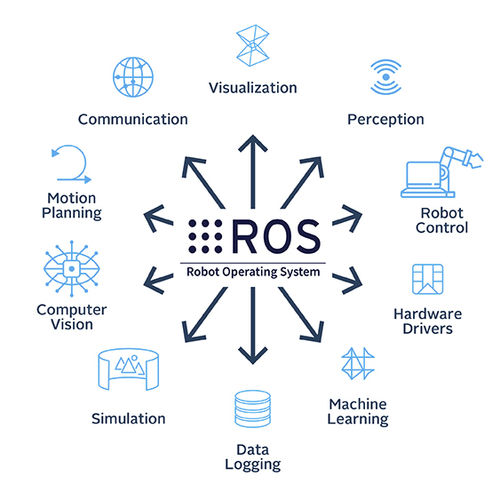
\includegraphics[scale=0.20]{figuras/ros_aplicaciones.jpg}
        \caption{Framework de \acrshort{ROS}}
        \label{fig:ros_aplicaciones}
    \end{subfigure}
    \begin{subfigure}[h!]{0.45\linewidth} 
        \centering
        
\includegraphics[scale=1.6]{figuras/ros2-humble-small.png}
        \caption{Versión de ROS2 de este proyecto \cite{ROS2_docu_humble}}
        \label{fig:ros2-humble-small}
    \end{subfigure}
    \caption{Limitaciones de la \acrshort{AM} tradicional}
\end{figure}

\subsection{Motivación del proyecto}
Siguiendo la línea descrita por la sección \ref{seccion: Limitaciones}, se ha visto que existen multitud de métodos de calibración extrínseca para una estación de fabricación robotizada. En todos ellos se ha visto que la tendencia actual apunta hacia la inclusión de procesos de calibración que además incluyan un sistema de aprendizaje offline. Esto es, que también se simulen rápidamente las operaciones planteadas para el robot. 

Es fundamental establecer un proceso de preparación de la estación de trabajo en el que se pueda obtener de forma eficaz la definición de sus sistemas de referencia fundamentales. En otras palabras, se necesita operar grandes cantidades de datos de forma distribuida que permitan caracterizar geométrica y mecánicamente la mesa de trabajo, la herramienta empleada o las trayectorias a efectuar por el robot.

Como se ha visto anteriormente, la inclusión de únicamente las herramientas proporcionadas por el fabricante del robot no resulta suficiente para este tipo de aplicaciones. Por lo que el sistema de preparación debe contar con parámetros en tiempo real como la inclinación de la mesa, la presencia de elementos móviles o la temperatura del material depositado.

En este proyecto se propone un sistema de preparación de la estación de fabricación que integre estas funciones dentro de una interfaz amigable para el usuario y que pueda sintetizar un flujo de trabajo sencillo y modularizado. Para ello se definirá una estrategia de calibración offline de la estación, mientras se evalúan una serie de parámetros en tiempo real como puede ser la temperatura de la cama de impresión. 

Para solventar la capacidad de gestión de datos del robot -que resulta insuficiente para el objetivo de la estación- se plantea la integración de una arquitectura en \acrshort{ROS}2 con un computador externo efectuando otras tareas de forma simultánea. La introducción de ROS2 como entorno de trabajo frente a ROS, tiene la intención de servir como base para futuros desarrollos en los que se puedan definir (1) nuevas herramientas de cálculo de trayectorias usando la programación cruzada entre Python y C++, (2) una modularización de tareas por parte del robot y (3) la posibilidad de establecer comunicaciones en el futuro con elementos de una arquitectura de comunicaciones distribuida.

\section{Marco del proyecto} \label{section:  marco del proyecto}
Este proyecto se ha desarrollado dentro de un entorno multidisciplinar más grande. El objetivo a largo plazo de este equipo es el diseño y construcción de una estación de fabricación aditiva robotizada centrada en los procesos \acrshort{NPAM}. El proceso abarcado se puede definir a través de tres etapas:
\begin{enumerate}
    \item \textbf{Planificación de producto:} Es la parte correspondiente al diseño de piezas que pasarán a la estación de fabricación. En ella se busca implementar un algoritmo de slicing automatizado \cite{paper_Q1_Alvaro_Adrian} que permita obtener un conjunto de puntos cartesianos en el espacio que definan la pieza resultante final. Amparo Sancho en su trabajo anterior \cite{TFM_SanchoAmparo} estableció una primera versión de este proceso y es la que se ha usado como referencia principal.
    \item \textbf{Preparación de estación:} Esta etapa comprende las operaciones de calibración del brazo robótico empleado y calentamiento del extrusor y la cama de impresión. En esta fase del proceso general es donde se encuentra ubicado este proyecto.
    \item \textbf{Operación de manufactura:} Es la fase final del proceso. En ella se da luz verde para que una vez la cama y el extrusor se encuentren a las temperaturas deseadas, el brazo robótico comience a efectuar la trayectoria calculada para obtener el producto definido en la fase de planificación.
\end{enumerate}

Los materiales aportados para el diseño y montaje de la estación han sido aportados por el grupo de \href{https://fabricacion.industriales.upm.es/}{Ingeniería de Fabricación} de la \href{https://www.industriales.upm.es/}{ETSII-UPM}. Dentro de todos los componentes utilizados destaca el robot UR10 ubicado en el laboratorio del grupo junto a una mesa de trabajo especialmente diseñada para su operación.

\begin{figure}[h!]
    \centering
    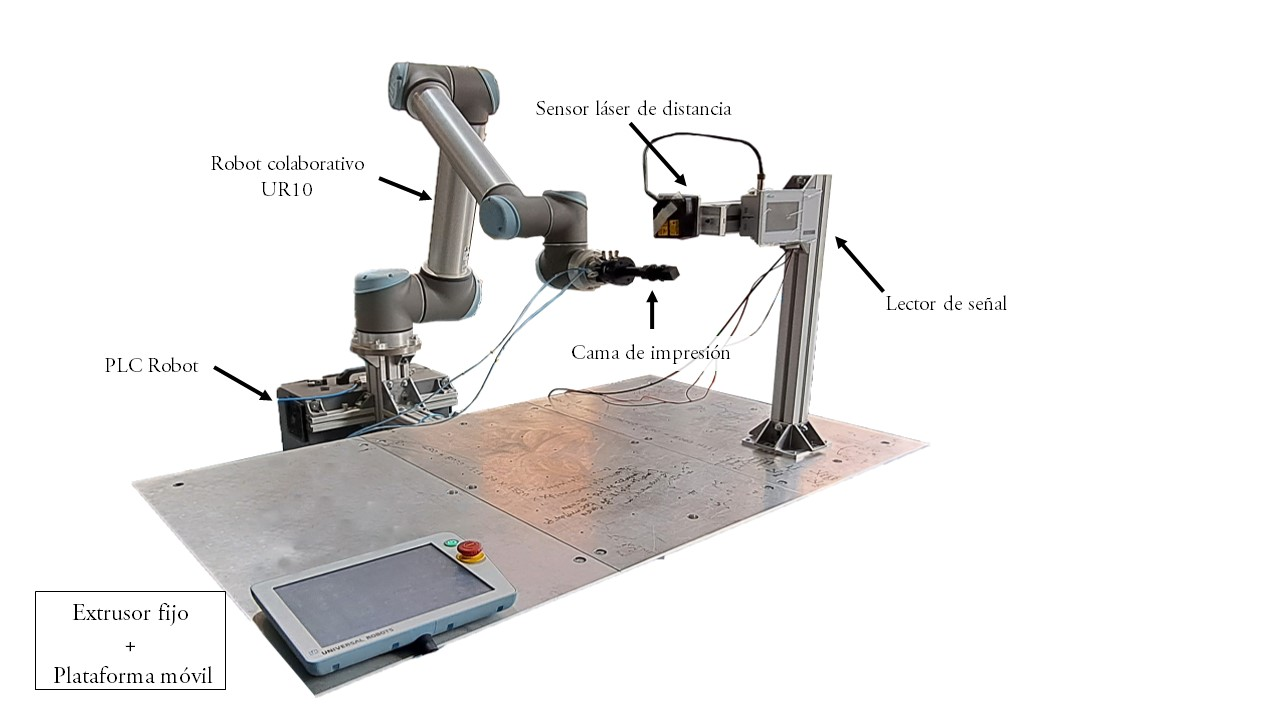
\includegraphics[scale=0.30]{figuras/estacion_NPAM_sin_estruxor.JPG}
    \caption{Versión inicial de la estación}
    \label{fig: estacion_NPAM_sin_estruxor}
\end{figure}

Se desea que la estación tenga la cama acoplada al \acrshort{TCP} y el extrusor se encuentre ubicado en una posición fija con la finalidad de asegurar que el material extruído se deposite en la dirección de la gravedad. Esta configuración también es útil para ampliar el diseño de plataformas de impresión personalizadas, de modo que sea posible aprovechar más los \acrshort{DOF} proporcionados por el manipulador robótico. De cara a soluciones más convencionales, esta configuración resulta ventajosa para evitar introducir grados de libertad extra relacionados con la configuración de la mesa o el soporte de la estación. 

La Figura \ref{fig: estacion_NPAM_sin_estruxor} muestra una versión inicial de la estación \acrshort{NPAM} y se sitúa aproximadamente por el mes de Octubre de 2023. Esta versión incluye un sensor láser para tomar medidas de calibración de la cama del robot y ha sido utilizada en trabajos de fin de titulación previos \cite{TFM_SanchoAmparo} \cite{TFM_Lu}.

La cama cuenta con su propio diseño realizado por Iñaki Echepare \cite{TFM_IñakiEchepare} y se caracteriza por contar con un cartucho calefactor en su interior que puede activarse a conectándolo a un circuito electrónico. El soporte para el extrusor ha sido diseñado por Adrián Martínez. 

Tanto los datos de temperatura de la cama de impresión como del extrusor, deben retransmitirse de forma continuada a una unidad de control. En el caso de la temperatura de la cama, los mensajes y el bucle de control han sido definidos en colaboración con Irene Rodríguez.

Este macroproyecto integra labores variadas de cálculos cinemáticos, conocimientos de automatización, comunicaciones industriales, electrónica o ensayos de mecánica de materiales. Es decir, tiene un alcance transversal y necesita la colaboración de equipos multidisciplinares. En otras palabras y como punto adicional de este trabajo, se ha establecido un marco de coordinación entre algunos de los equipos partícipes en el diseño y construcción de la estación robotizada. En concreto se han establecido las interfaces de comunicación entre arquitecturas software y de operación hardware, así como también se ha creado un \href{\linkrepositorio}{repositorio} donde se ubica un manual de conocimiento básico del proyecto en forma de wiki  \cite{repo_github_TFM_MiguelLerinAlonso}.

La Figura \ref{fig:areas_macroproyecto} muestra las diferentes áreas que conforman este macroproyecto\footnote{Una versión con los nombres de los alumnos involucrados en cada tarea se dispone en la Figura \ref{fig:marco proyecto tareas y autor} del apéndice \ref{cap: anexo marco proyecto}.}, se marcan en color rojo aquellas en las que este trabajo tiene un papel principal. Estas tareas entran dentro de tres campos principales: la arquitectura informática de la máquina, la planificación de procesos y generación de trayectorias; y la preparación de de procesos. Las tareas efectuadas dentro del área de arquitectura informática fueron aquellas relacionadas con la creación de una interfaz de usuario de ROS2 para el manejo y operación de la estación. Las correspondientes a la planificación de procesos y generación de trayectorias de buscaban definir un nuevo flujo de trabajo para la estación e integrarlo con los equipos ya existentes y los de nuevo desarrollo. Finalmente, se realizaba una tarea de calibración del robot dentro del área de preparación de procesos.

\begin{figure}[h!]
    \centering
    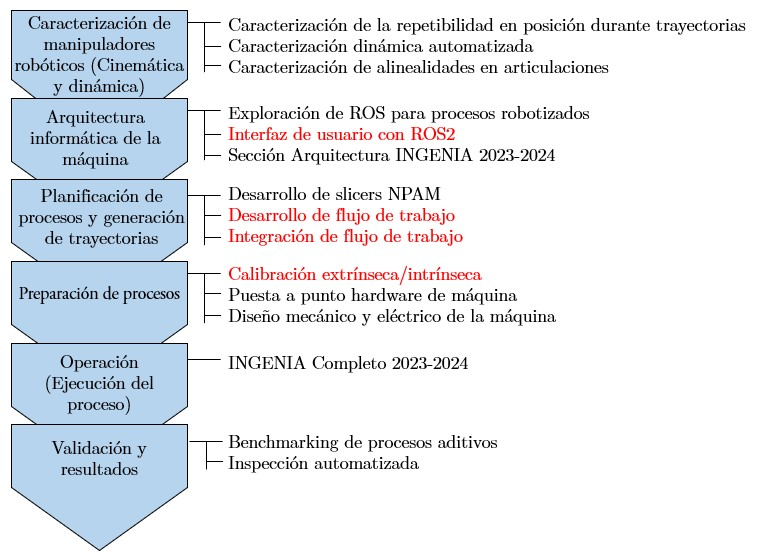
\includegraphics[scale=0.65]{figuras/marco_proyecto_solo_tareas_v2.jpg}
    \caption{Áreas del macroproyecto en el que se integra este trabajo}
    \label{fig:areas_macroproyecto}
\end{figure}

La Figura \ref{fig:ambitos_coordinacion} establece una representación visual de los ámbitos de coordinación llevados durante este proyecto. Como puede observarse, a parte del presente trabajo existen cinco equipos especializados que colaboran activamente entre sí. Los equipos están formados por otros alumnos que se encuentran trabajando en sus respectivos trabajos de fin de titulación y alumnos del curso 2023-2024 de la asignatura \href{http://fabricacion.industriales.upm.es/2022/09/06/asignatura-ingenia-diseno-de-estacion-colaborativa-4-0/}{INGENIA Diseño de sistemas inteligentes con robots y AGV} \cite{web_INGENIA}. La labor de dichos equipos y su conexión con el presente proyecto se describen en las siguientes lineas:

\begin{itemize}
    \item \textbf{Generación de trayectorias:} Equipo responsable de programación del software de slicing empleado para el procesamiento de modelos \acrshort{CAD} que desean ser impresos. Este equipo aporta al proyecto un archivo CSV en el que se encuentran definidos el conjunto de puntos asociados a un sistema referencia que debe recorrer el manipulador robótico. Es decir, aporta los datos de entrada para el sistema de cálculo configuraciones cinemáticas del robot UR.
    \item \textbf{\acrshort{DfAM}:} Este equipo es el responsable de plantear y evaluar aquellas técnicas de diseño mecánico que pueden ser de mejor resultado para los requisitos de la estación. Deben tener en cuenta el tipo de producto que se desea fabricar a través del proceso \acrshort{NPAM} y trabajar junto a la sección de Generación de trayectorias para hallar el procedimiento óptimo de orientación y fabricación de la pieza objetivo. Es decir, los componentes de este equipo se encargan de valorar la integración de otras tecnologías en el resultado final como pueden ser metodologías multimaterial o con optimización topológica.
    \item \textbf{Diseño mecánico y eléctrico:} Los integrantes de esta sección han sido responsables de la elaboración del soporte que aloja el extrusor de material. Esta sección está en contacto constante con \acrshort{DfAM} para valorar la energía y flujo de material que demanda la pieza resultado del proceso \acrshort{NPAM}. Sigue el proceder con la sección de Actuadores máquina para especificar la alimentación eléctrica que deben proveer a los actuadores de la máquina.
    \item \textbf{Actuadores máquina:} Está sección es la encargada de establecer integrar y establecer los bucles de control que relacionan a los actuadores de la estación \acrshort{NPAM} robotizada. Esta labor la hacen en colaboración con el equipo de Arquitectura para mejorar el tratamiento de los sensores y actuadores, y siguen las directrices indicadas por el diseño de la arquitectura informática realizada en este trabajo. Los equipos de sensorizado y actuación más relevantes para sus integrantes han sido el control de temperatura asociado a la cama de impresión y la regulación del extrusor de material en cuanto a flujo de alimentación y modelado térmico.
    \item \textbf{Arquitectura:} Son los responsables de la definición de movimientos del robot UR a través de un conjunto de aplicaciones software que deben también monitorizar sus variables internas. Reciben el conjunto de puntos definido por el software de slicing de la sección de Generación de trayectorias y se encuentran en conversaciones continuadas con el equipo de actuadores máquinas para definir el conjunto de mensajes entre equipos y su tratamiento. También colaboran en este proyecto en labores de optimización de código, pruebas de ejecución en tiempo real o la definición del espacio de trabajo virtualizado.
\end{itemize}

\begin{figure}[h!]
    \centering
    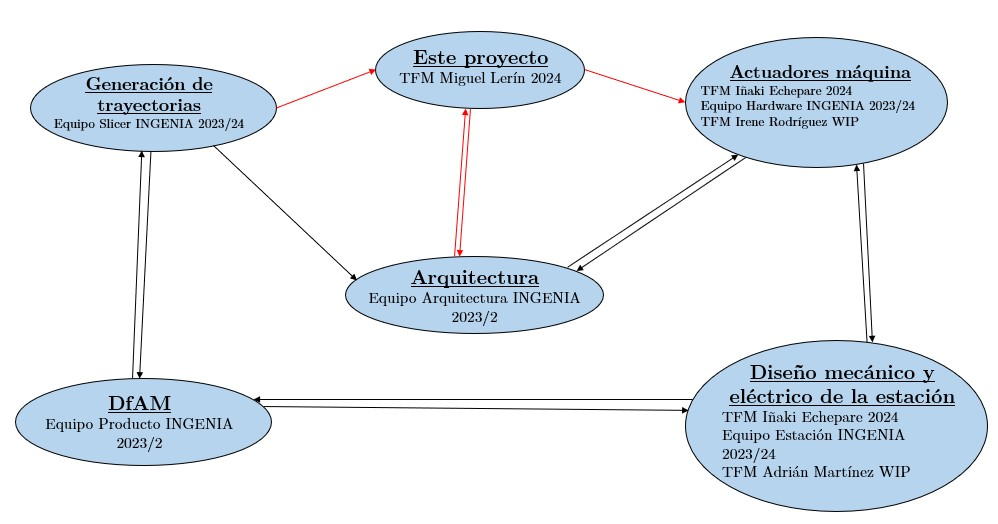
\includegraphics[scale=0.6]{figuras/ambitos_coordinacion_1_esquema_v2.jpg}
    \caption{Ámbitos de coordinación llevados durante la ejecución del trabajo}
    \label{fig:ambitos_coordinacion}
\end{figure}

\phantom{Este texto no se verá, pero ocupará espacio. Lo uso para que la figura de los ámbitos de coordinación quede al comienzo de la página}